% Options for packages loaded elsewhere
% Options for packages loaded elsewhere
\PassOptionsToPackage{unicode}{hyperref}
\PassOptionsToPackage{hyphens}{url}
\PassOptionsToPackage{dvipsnames,svgnames,x11names}{xcolor}
%
\documentclass[
  letterpaper,
  DIV=11,
  numbers=noendperiod]{scrartcl}
\usepackage{xcolor}
\usepackage{amsmath,amssymb}
\setcounter{secnumdepth}{-\maxdimen} % remove section numbering
\usepackage{iftex}
\ifPDFTeX
  \usepackage[T1]{fontenc}
  \usepackage[utf8]{inputenc}
  \usepackage{textcomp} % provide euro and other symbols
\else % if luatex or xetex
  \usepackage{unicode-math} % this also loads fontspec
  \defaultfontfeatures{Scale=MatchLowercase}
  \defaultfontfeatures[\rmfamily]{Ligatures=TeX,Scale=1}
\fi
\usepackage{lmodern}
\ifPDFTeX\else
  % xetex/luatex font selection
\fi
% Use upquote if available, for straight quotes in verbatim environments
\IfFileExists{upquote.sty}{\usepackage{upquote}}{}
\IfFileExists{microtype.sty}{% use microtype if available
  \usepackage[]{microtype}
  \UseMicrotypeSet[protrusion]{basicmath} % disable protrusion for tt fonts
}{}
\makeatletter
\@ifundefined{KOMAClassName}{% if non-KOMA class
  \IfFileExists{parskip.sty}{%
    \usepackage{parskip}
  }{% else
    \setlength{\parindent}{0pt}
    \setlength{\parskip}{6pt plus 2pt minus 1pt}}
}{% if KOMA class
  \KOMAoptions{parskip=half}}
\makeatother
% Make \paragraph and \subparagraph free-standing
\makeatletter
\ifx\paragraph\undefined\else
  \let\oldparagraph\paragraph
  \renewcommand{\paragraph}{
    \@ifstar
      \xxxParagraphStar
      \xxxParagraphNoStar
  }
  \newcommand{\xxxParagraphStar}[1]{\oldparagraph*{#1}\mbox{}}
  \newcommand{\xxxParagraphNoStar}[1]{\oldparagraph{#1}\mbox{}}
\fi
\ifx\subparagraph\undefined\else
  \let\oldsubparagraph\subparagraph
  \renewcommand{\subparagraph}{
    \@ifstar
      \xxxSubParagraphStar
      \xxxSubParagraphNoStar
  }
  \newcommand{\xxxSubParagraphStar}[1]{\oldsubparagraph*{#1}\mbox{}}
  \newcommand{\xxxSubParagraphNoStar}[1]{\oldsubparagraph{#1}\mbox{}}
\fi
\makeatother


\usepackage{longtable,booktabs,array}
\newcounter{none} % for unnumbered tables
\usepackage{calc} % for calculating minipage widths
% Correct order of tables after \paragraph or \subparagraph
\usepackage{etoolbox}
\makeatletter
\patchcmd\longtable{\par}{\if@noskipsec\mbox{}\fi\par}{}{}
\makeatother
% Allow footnotes in longtable head/foot
\IfFileExists{footnotehyper.sty}{\usepackage{footnotehyper}}{\usepackage{footnote}}
\makesavenoteenv{longtable}
\usepackage{graphicx}
\makeatletter
\newsavebox\pandoc@box
\newcommand*\pandocbounded[1]{% scales image to fit in text height/width
  \sbox\pandoc@box{#1}%
  \Gscale@div\@tempa{\textheight}{\dimexpr\ht\pandoc@box+\dp\pandoc@box\relax}%
  \Gscale@div\@tempb{\linewidth}{\wd\pandoc@box}%
  \ifdim\@tempb\p@<\@tempa\p@\let\@tempa\@tempb\fi% select the smaller of both
  \ifdim\@tempa\p@<\p@\scalebox{\@tempa}{\usebox\pandoc@box}%
  \else\usebox{\pandoc@box}%
  \fi%
}
% Set default figure placement to htbp
\def\fps@figure{htbp}
\makeatother


% definitions for citeproc citations
\NewDocumentCommand\citeproctext{}{}
\NewDocumentCommand\citeproc{mm}{%
  \begingroup\def\citeproctext{#2}\cite{#1}\endgroup}
\makeatletter
 % allow citations to break across lines
 \let\@cite@ofmt\@firstofone
 % avoid brackets around text for \cite:
 \def\@biblabel#1{}
 \def\@cite#1#2{{#1\if@tempswa , #2\fi}}
\makeatother
\newlength{\cslhangindent}
\setlength{\cslhangindent}{1.5em}
\newlength{\csllabelwidth}
\setlength{\csllabelwidth}{3em}
\newenvironment{CSLReferences}[2] % #1 hanging-indent, #2 entry-spacing
 {\begin{list}{}{%
  \setlength{\itemindent}{0pt}
  \setlength{\leftmargin}{0pt}
  \setlength{\parsep}{0pt}
  % turn on hanging indent if param 1 is 1
  \ifodd #1
   \setlength{\leftmargin}{\cslhangindent}
   \setlength{\itemindent}{-1\cslhangindent}
  \fi
  % set entry spacing
  \setlength{\itemsep}{#2\baselineskip}}}
 {\end{list}}
\usepackage{calc}
\newcommand{\CSLBlock}[1]{\hfill\break\parbox[t]{\linewidth}{\strut\ignorespaces#1\strut}}
\newcommand{\CSLLeftMargin}[1]{\parbox[t]{\csllabelwidth}{\strut#1\strut}}
\newcommand{\CSLRightInline}[1]{\parbox[t]{\linewidth - \csllabelwidth}{\strut#1\strut}}
\newcommand{\CSLIndent}[1]{\hspace{\cslhangindent}#1}



\setlength{\emergencystretch}{3em} % prevent overfull lines

\providecommand{\tightlist}{%
  \setlength{\itemsep}{0pt}\setlength{\parskip}{0pt}}



 


\KOMAoption{captions}{tableheading}
\makeatletter
\@ifpackageloaded{caption}{}{\usepackage{caption}}
\AtBeginDocument{%
\ifdefined\contentsname
  \renewcommand*\contentsname{Table of contents}
\else
  \newcommand\contentsname{Table of contents}
\fi
\ifdefined\listfigurename
  \renewcommand*\listfigurename{List of Figures}
\else
  \newcommand\listfigurename{List of Figures}
\fi
\ifdefined\listtablename
  \renewcommand*\listtablename{List of Tables}
\else
  \newcommand\listtablename{List of Tables}
\fi
\ifdefined\figurename
  \renewcommand*\figurename{Figure}
\else
  \newcommand\figurename{Figure}
\fi
\ifdefined\tablename
  \renewcommand*\tablename{Table}
\else
  \newcommand\tablename{Table}
\fi
}
\@ifpackageloaded{float}{}{\usepackage{float}}
\floatstyle{ruled}
\@ifundefined{c@chapter}{\newfloat{codelisting}{h}{lop}}{\newfloat{codelisting}{h}{lop}[chapter]}
\floatname{codelisting}{Listing}
\newcommand*\listoflistings{\listof{codelisting}{List of Listings}}
\makeatother
\makeatletter
\makeatother
\makeatletter
\@ifpackageloaded{caption}{}{\usepackage{caption}}
\@ifpackageloaded{subcaption}{}{\usepackage{subcaption}}
\makeatother
\usepackage{bookmark}
\IfFileExists{xurl.sty}{\usepackage{xurl}}{} % add URL line breaks if available
\urlstyle{same}
\hypersetup{
  pdftitle={Sesión introductoria},
  pdfauthor={Oscar Bustos},
  colorlinks=true,
  linkcolor={blue},
  filecolor={Maroon},
  citecolor={Blue},
  urlcolor={Blue},
  pdfcreator={LaTeX via pandoc}}


\title{Sesión introductoria}
\usepackage{etoolbox}
\makeatletter
\providecommand{\subtitle}[1]{% add subtitle to \maketitle
  \apptocmd{\@title}{\par {\large #1 \par}}{}{}
}
\makeatother
\subtitle{Técnicas de aprendizaje de máquina}
\author{Oscar Bustos}
\date{}
\begin{document}
\maketitle


\section{Presentación}\label{presentaciuxf3n}

\subsection{¡Presenta a tu Socio!}\label{presenta-a-tu-socio}

¡Hola a todos!

Comparte lo siguiente sobre tu socio:

\textbf{Nombre}, semestre, su \textbf{profesión ideal}, dónde les
gustaría \textbf{emprender} y qué les llama la \textbf{atención} sobre
esta clase.

\subsection{Estadísticas de Clase}\label{estaduxedsticas-de-clase}

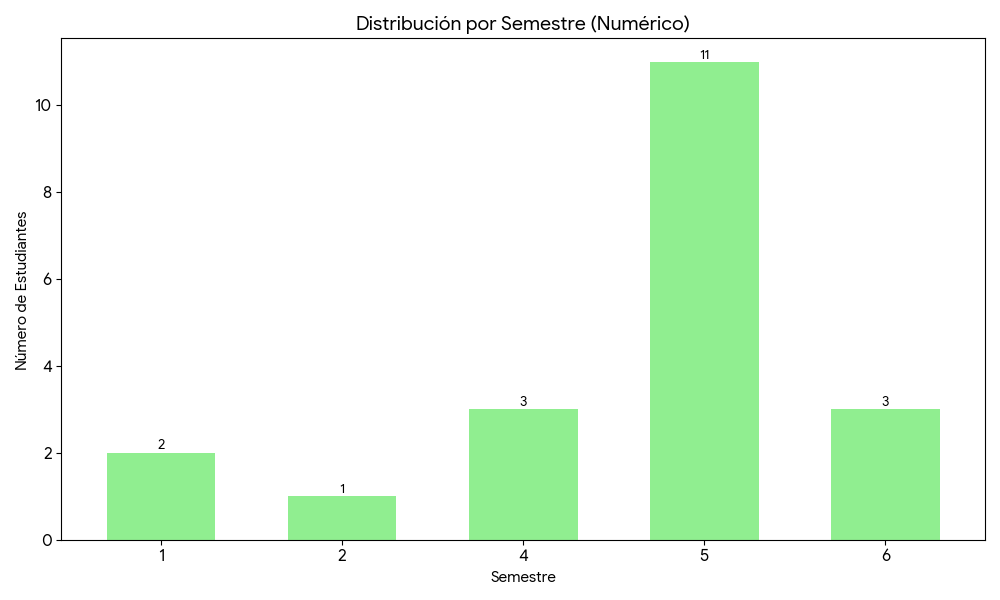
\includegraphics[width=0.45\linewidth,height=\textheight,keepaspectratio]{assets/SemestreStats.png}

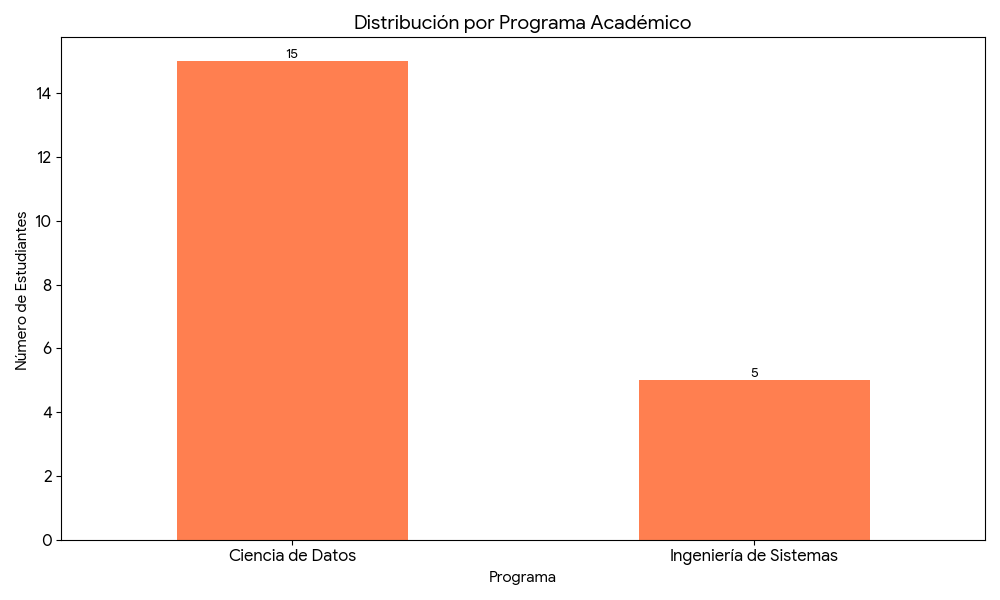
\includegraphics[width=0.45\linewidth,height=\textheight,keepaspectratio]{assets/ProgramStats.png}

\subsection{¡Conozcámonos!}\label{conozcuxe1monos}

\begin{itemize}
\tightlist
\item
  Soy Oscar Bustos
\item
  Ingeniero Metratrónico, PhD. (c) en Ingeniería - PUJ
\item
  Docente Javeriano, Tech Manager en Mercadolibre
\item
  Me gusta todo lo relacionado con IA / Advanced Analytics
\end{itemize}

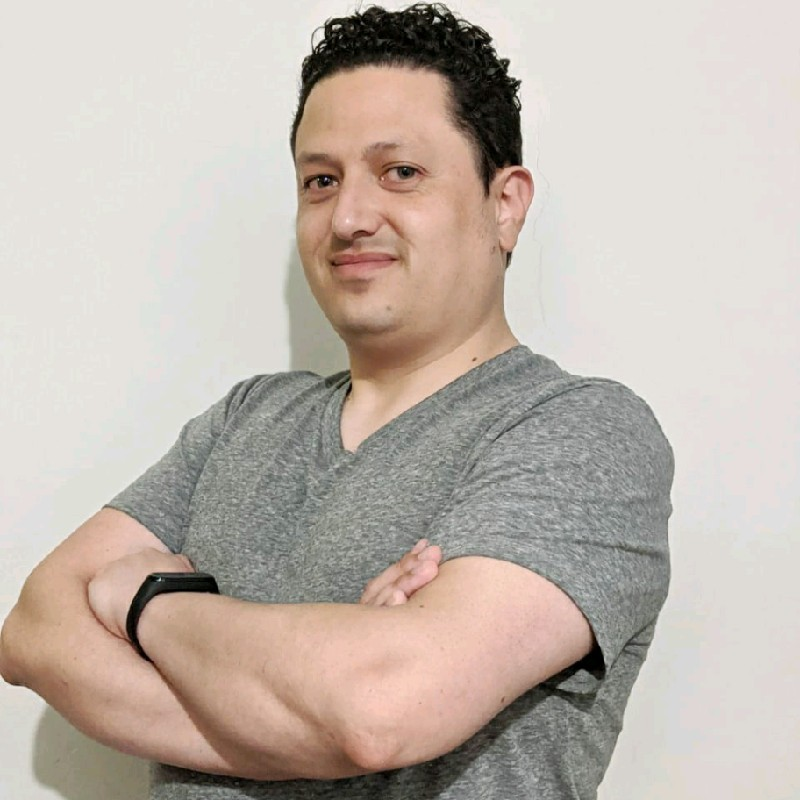
\includegraphics[width=1\linewidth,height=\textheight,keepaspectratio]{assets/FotoReciente.png}

\section{Evaluación y Logística}\label{evaluaciuxf3n-y-loguxedstica}

\subsection{Estructura del Curso}\label{estructura-del-curso}

\begin{itemize}
\tightlist
\item
  \textbf{Exposición}

  \begin{itemize}
  \tightlist
  \item
    Exposición 10\%
  \end{itemize}
\item
  \textbf{Talleres}

  \begin{itemize}
  \tightlist
  \item
    Talleres 40\%
  \item
    Un taller por clase
  \end{itemize}
\item
  \textbf{Proyecto Final}

  \begin{itemize}
  \tightlist
  \item
    Entrega 1: 25\%
  \item
    Entrega 2: 25\%
  \end{itemize}
\end{itemize}

\subsection{Reglas}\label{reglas}

\begin{itemize}
\tightlist
\item
  Todas las clases tienen un \textbf{taller práctico} asociado, para
  entregar los domingos a las \textbf{11:59pm}
\item
  Los talleres se resuelven y se envían en \textbf{parejas}.
  \textbackslash{}
\item
  El proyecto en grupo debe ser integrado por \textbf{4 personas}, 2
  parejas idealmente. \textbackslash{}
\item
  Todas las entregas se hacen a través del \textbf{Campus Virtual}
  \textbackslash{}
\end{itemize}

\subsection{Reglas - Continuación}\label{reglas---continuaciuxf3n}

\begin{itemize}
\tightlist
\item
  Las clases empiezan a las \textbf{7:10am} y terminan a las
  \textbf{9:45am}, con un descanso de 15 minutos a las \textbf{8:30am}
\item
  Esta es una clase \textbf{amigable con la IA}. Se promueve el uso de
  la IA para la generación de código Python, para que el estudiante se
  enfoque en el análisis de los datos y de los modelos.
\item
  Para garantizar un ambiente agradable y libre de distracciones para
  todos, les agradecemos no fumar ni \textbf{vapear} en el salón de
  clase.
\item
  Con el fin de mantener la limpieza de nuestro espacio de trabajo, les
  solicitamos amablemente \textbf{no consumir alimentos} en el salón.
\end{itemize}

\subsection{Lecturas y Videos}\label{lecturas-y-videos}

\begin{itemize}
\tightlist
\item
  Todas las clases hay una lectura previa y un video recomendado
\item
  Todos los libros se encuentran en la plataforma de Springer Nature y
  O'Reilly
\item
  Se puede acceder a través de los recursos virtuales de la biblioteca
  en el siguiente enlace:
  \url{https://javeriana.libguides.com/az.php?a=o}
\end{itemize}

\subsection{Libros de la Clase}\label{libros-de-la-clase}

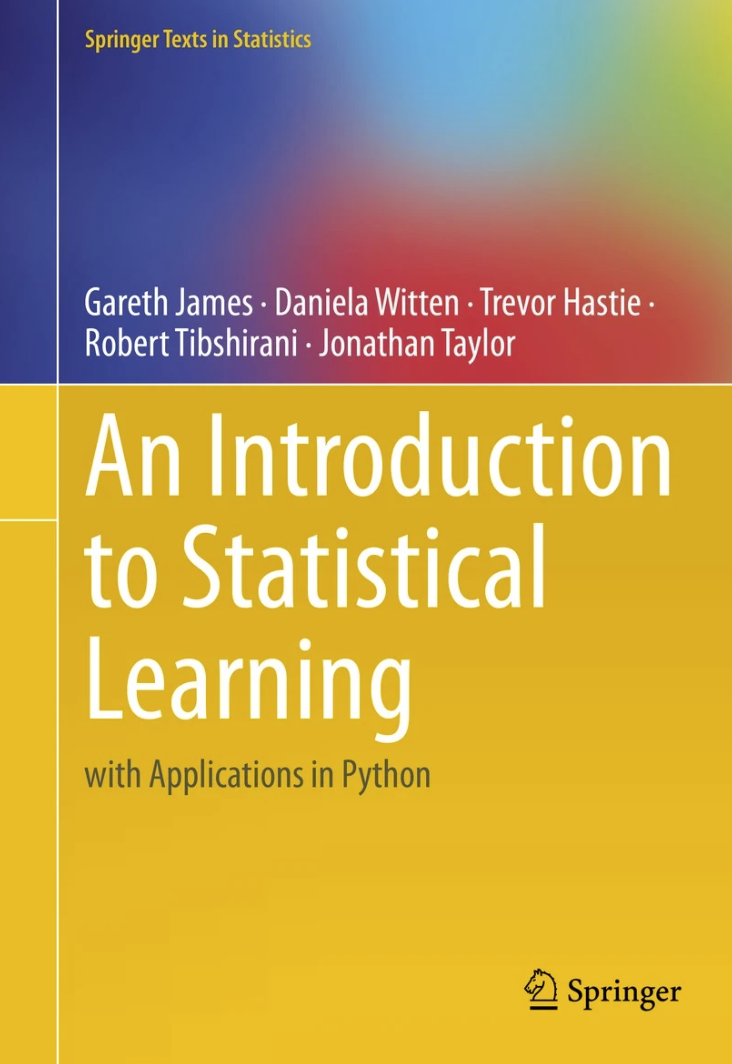
\includegraphics[width=0.3\linewidth,height=\textheight,keepaspectratio]{assets/IntroStatisticalLearning.png}\\
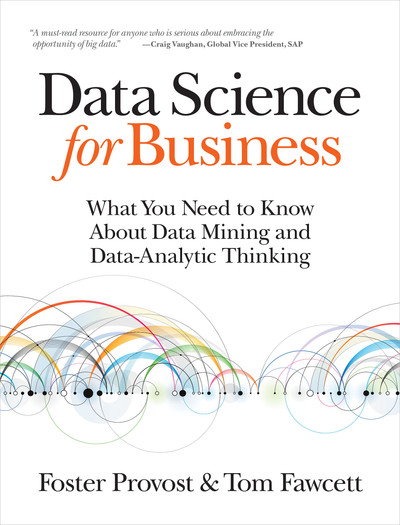
\includegraphics[width=0.3\linewidth,height=\textheight,keepaspectratio]{assets/DataScienceBusiness.jpg}

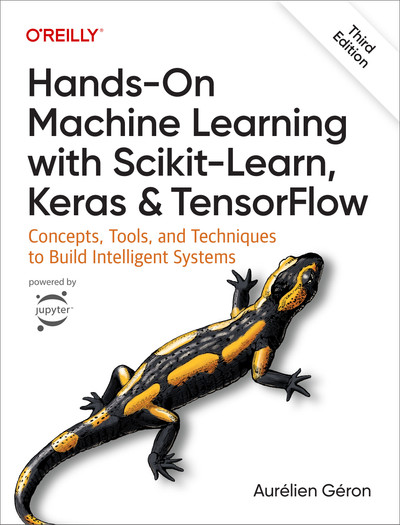
\includegraphics[width=0.3\linewidth,height=\textheight,keepaspectratio]{assets/keras.jpeg}

\subsection{Cronograma}\label{cronograma}

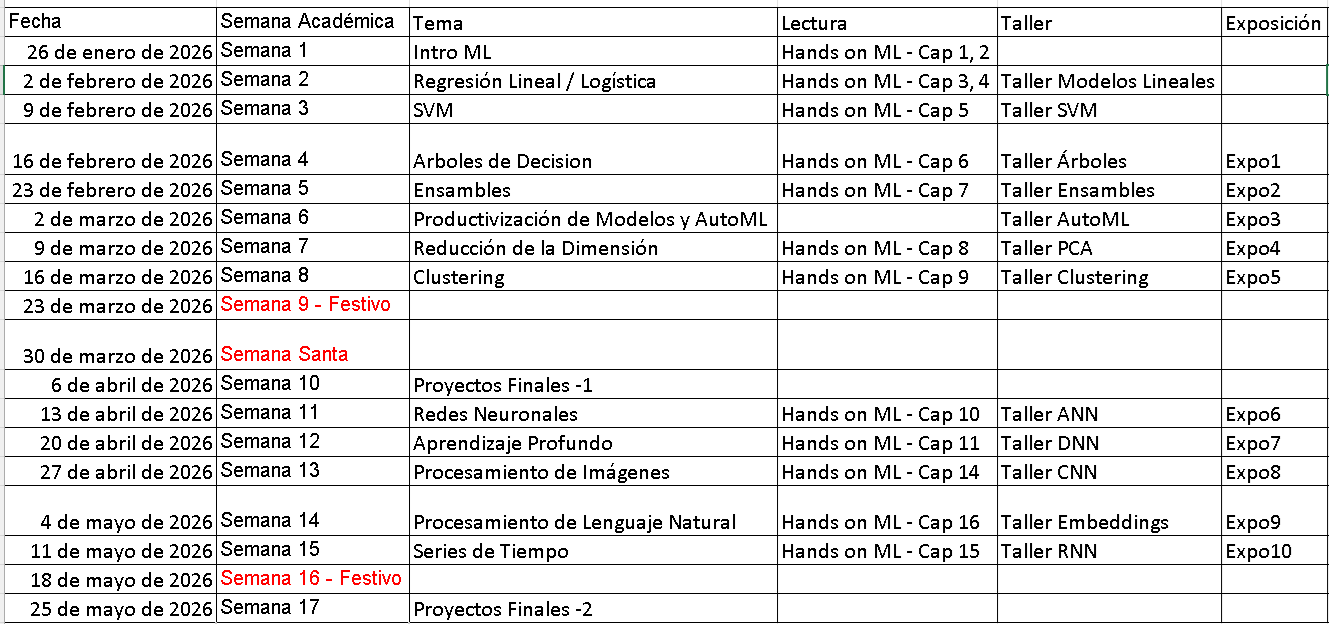
\includegraphics[width=1\linewidth,height=\textheight,keepaspectratio]{assets/CronogramaML.png}

\section{Motivación de la Clase}\label{motivaciuxf3n-de-la-clase}

\subsection{Definiciones}\label{definiciones}

\textbf{Pregunta}

\begin{itemize}
\tightlist
\item
  ¿Qué es inteligencia artificial?
\item
  ¿Qué es el aprendizaje de máquina?
\item
  ¿Qué es aprendizaje profundo?
\end{itemize}

\subsection{Definición de Inteligencia
Artificial}\label{definiciuxf3n-de-inteligencia-artificial}

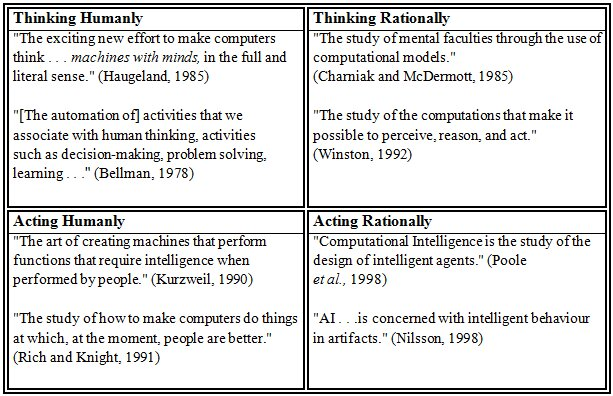
\includegraphics[width=0.6\linewidth,height=\textheight,keepaspectratio]{assets/DefinidioIA.jpg}
(Russell and Norvig 2020)

\subsection{Definición de Aprendizaje de
Máquina}\label{definiciuxf3n-de-aprendizaje-de-muxe1quina}

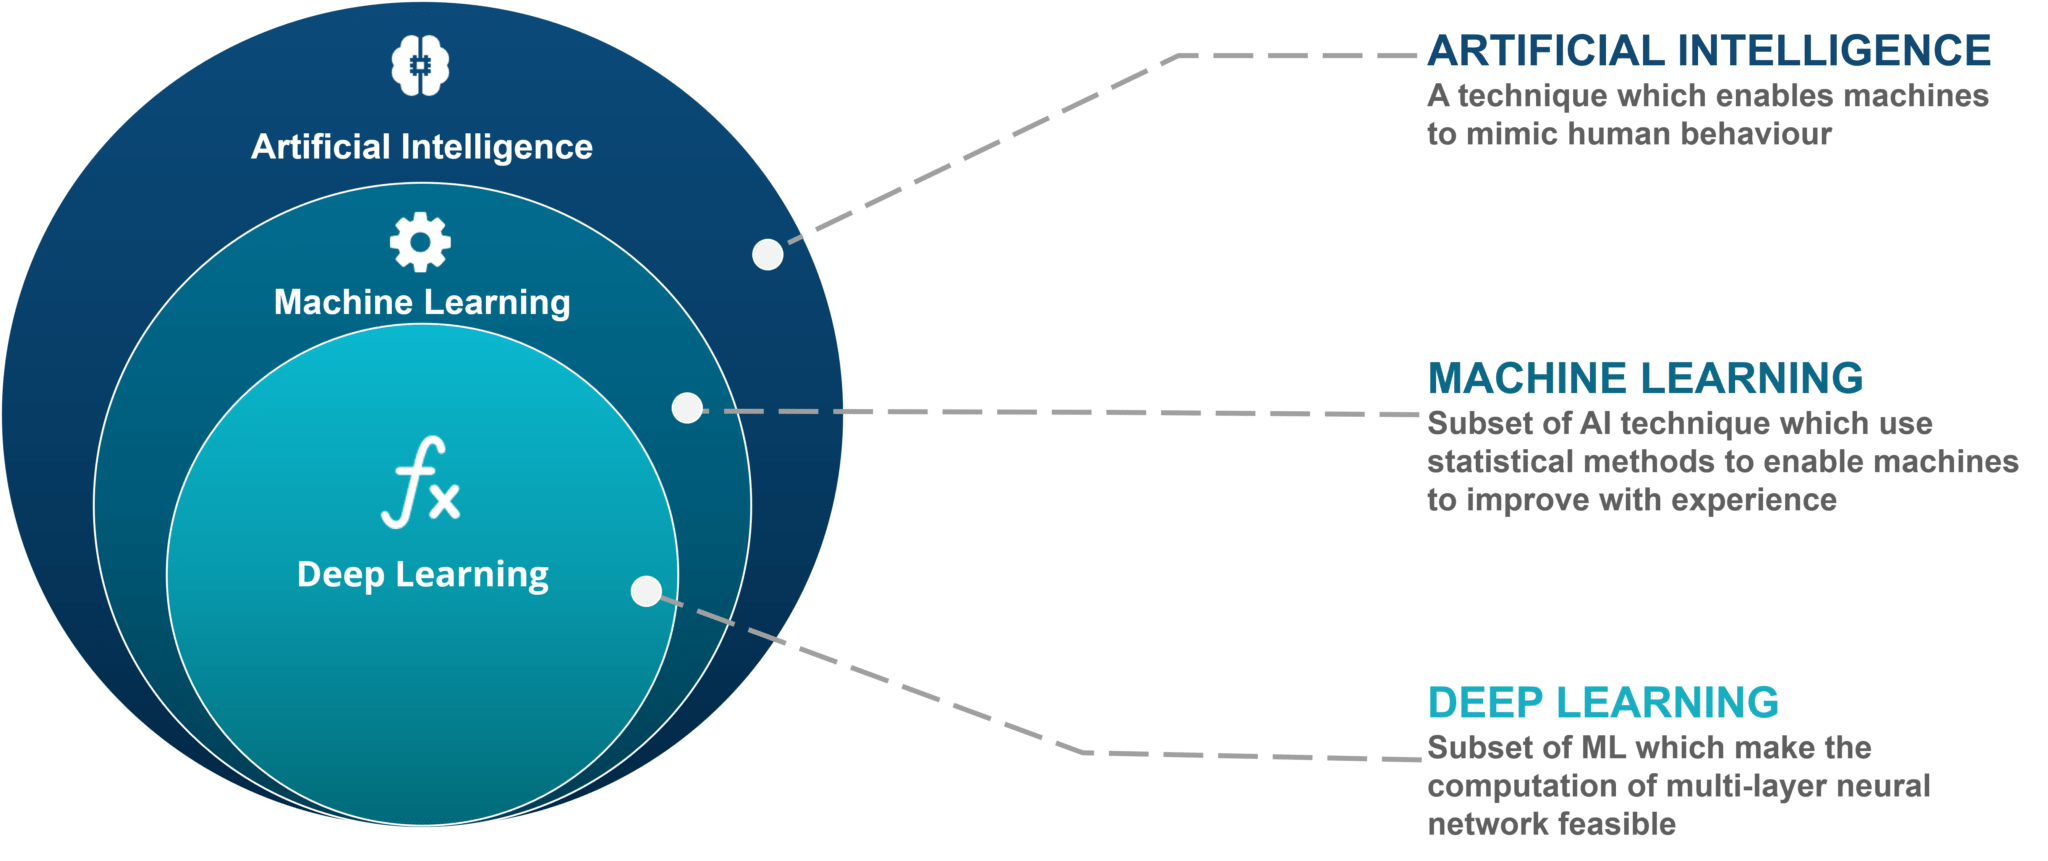
\includegraphics[width=0.8\linewidth,height=\textheight,keepaspectratio]{assets/AI-vs-ML-vs-Deep-Learning.png}
\url{https://www.edureka.co/blog/ai-vs-machine-learning-vs-deep-learning/}

\subsection{Aproximación Tradicional}\label{aproximaciuxf3n-tradicional}

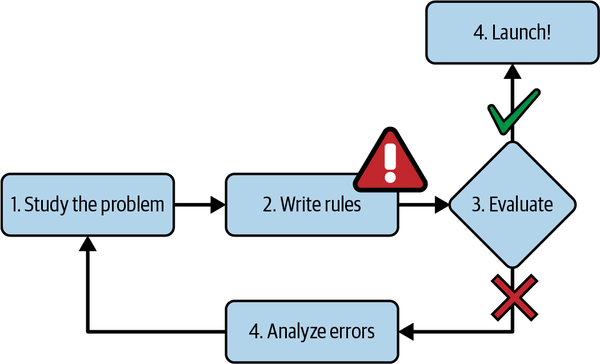
\includegraphics[width=0.6\linewidth,height=\textheight,keepaspectratio]{assets/mls3_0101.png}
\textbackslash{} (Géron 2022) Capítulo 1

\subsection{Aprendizaje de Máquina}\label{aprendizaje-de-muxe1quina}

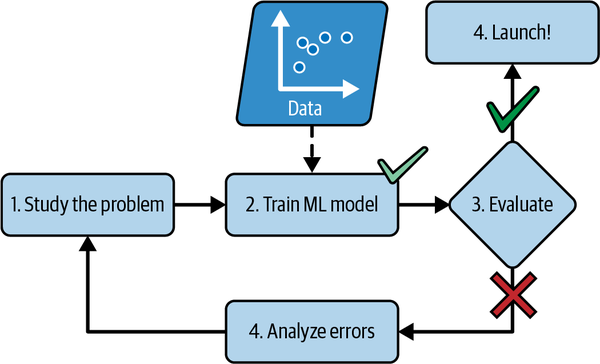
\includegraphics[width=0.6\linewidth,height=\textheight,keepaspectratio]{assets/mls3_0102.png}
\textbackslash{} (Géron 2022) Capítulo 1

\subsection{Aprendizaje de Máquina
Continuo}\label{aprendizaje-de-muxe1quina-continuo}

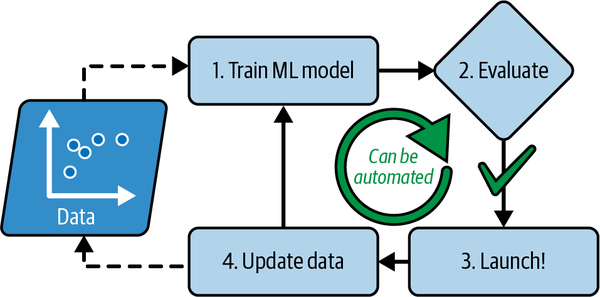
\includegraphics[width=0.6\linewidth,height=\textheight,keepaspectratio]{assets/mls3_0103.png}
\textbackslash{} (Géron 2022) Capítulo 1

\subsection{Historia de la IA}\label{historia-de-la-ia}

\textbf{Pregunta}

Si la IA ya existía en los años 50, ¿por qué hasta ahora estamos viendo
una clase sobre esto en la universidad como algo `nuevo'?

\url{https://www.mckinsey.com/capabilities/quantumblack/our-insights/an-executives-guide-to-ai}

\subsection{Roles Orientados a Datos - Data
Analyst}\label{roles-orientados-a-datos---data-analyst}

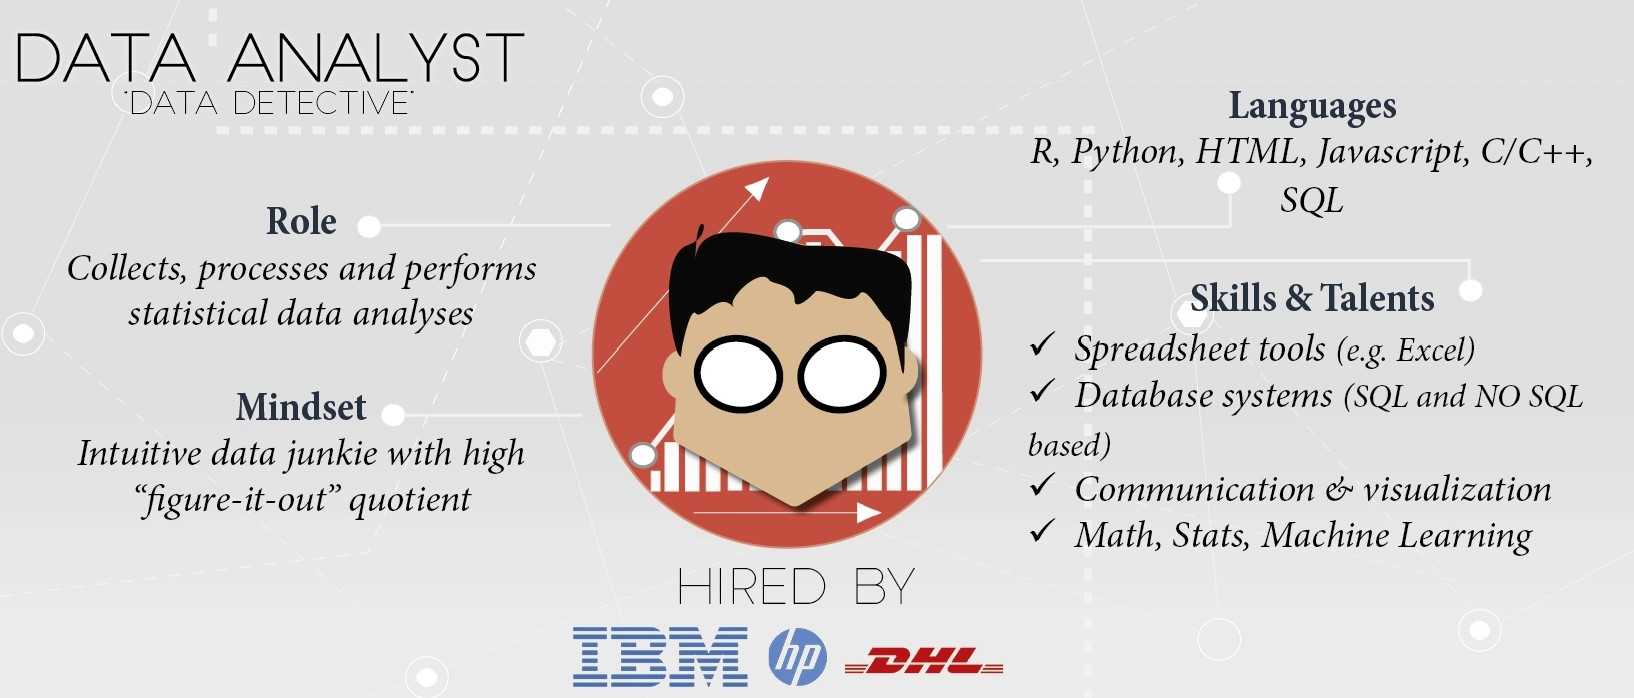
\includegraphics[width=1\linewidth,height=\textheight,keepaspectratio]{assets/dataAnalyst.jpg}
Tomado de:
\url{https://www.datacamp.com/tutorial/data-science-industry-infographic}

\subsection{Roles Orientados a Datos - Data
Analyst}\label{roles-orientados-a-datos---data-analyst-1}

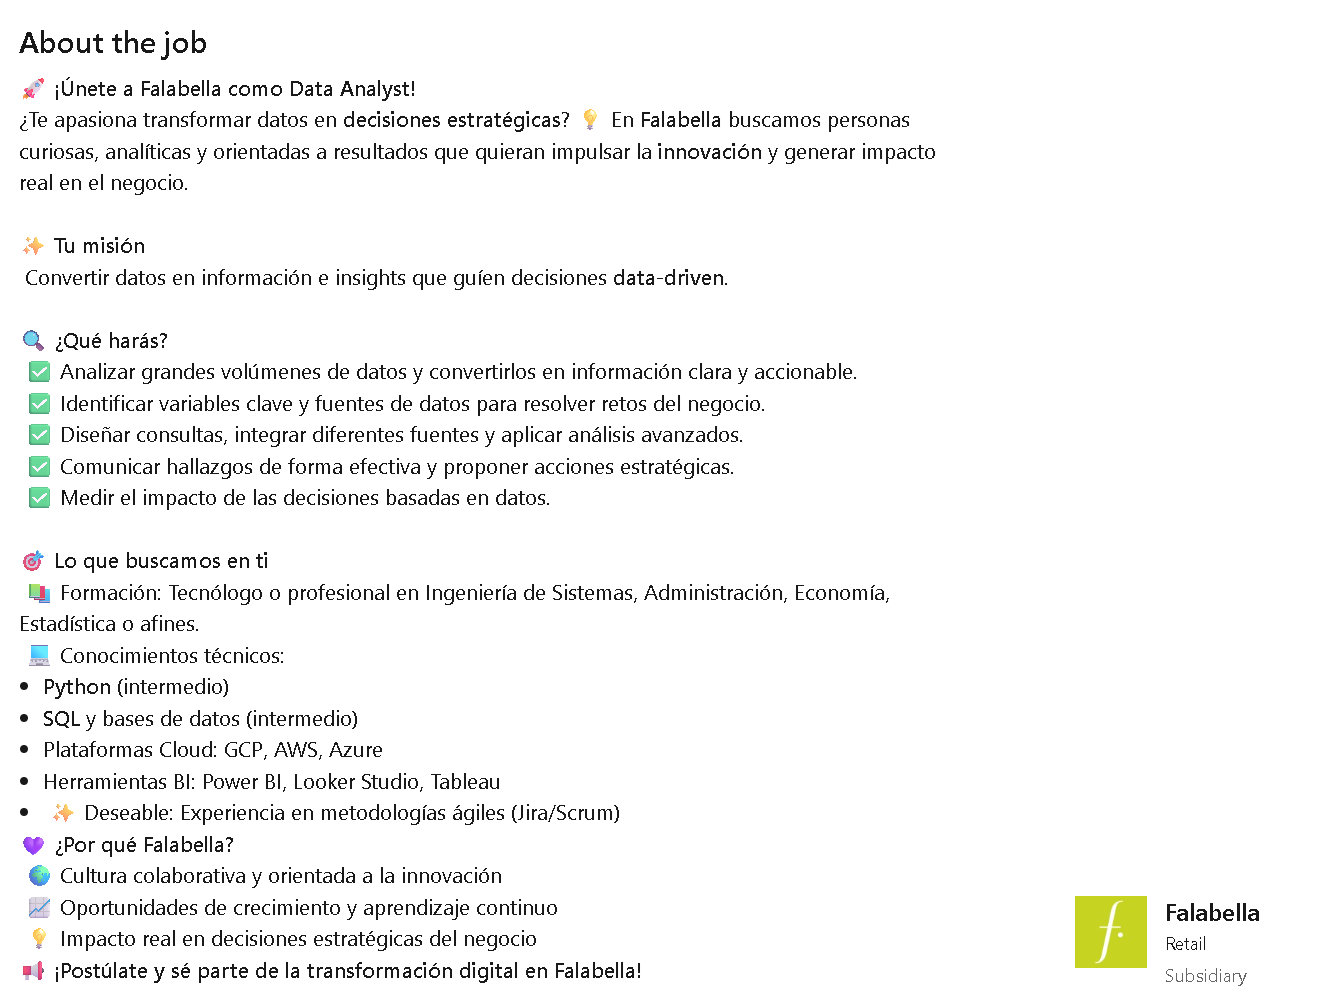
\includegraphics[width=0.6\linewidth,height=\textheight,keepaspectratio]{assets/TrabajoDataAnalyst.png}
Tomado de Linkedin

\subsection{Roles Orientados a Datos- Data
Scientist}\label{roles-orientados-a-datos--data-scientist}

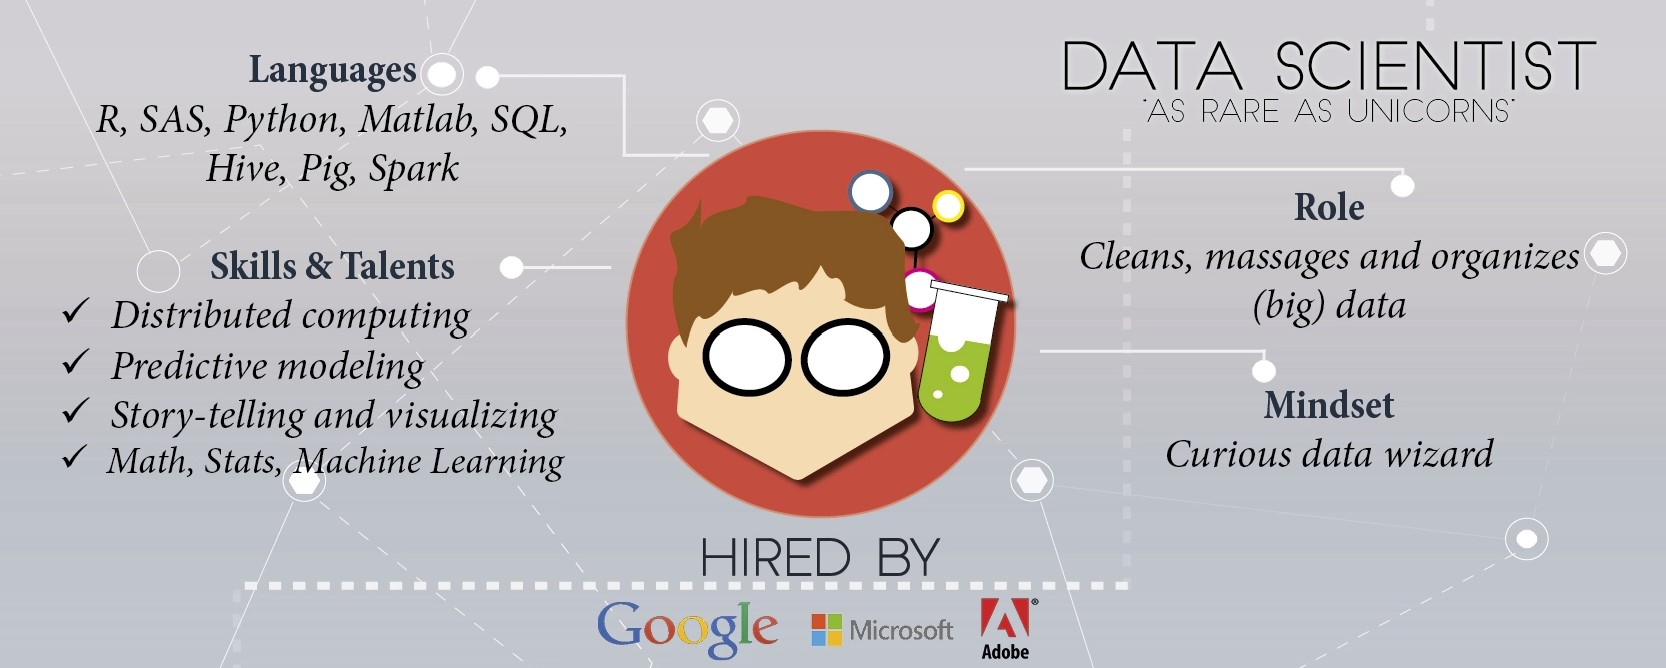
\includegraphics[width=1\linewidth,height=\textheight,keepaspectratio]{assets/dataScientist.jpg}
Tomado de:
\url{https://www.datacamp.com/tutorial/data-science-industry-infographic}

\subsection{Roles Orientados a Datos- Data
Scientist}\label{roles-orientados-a-datos--data-scientist-1}

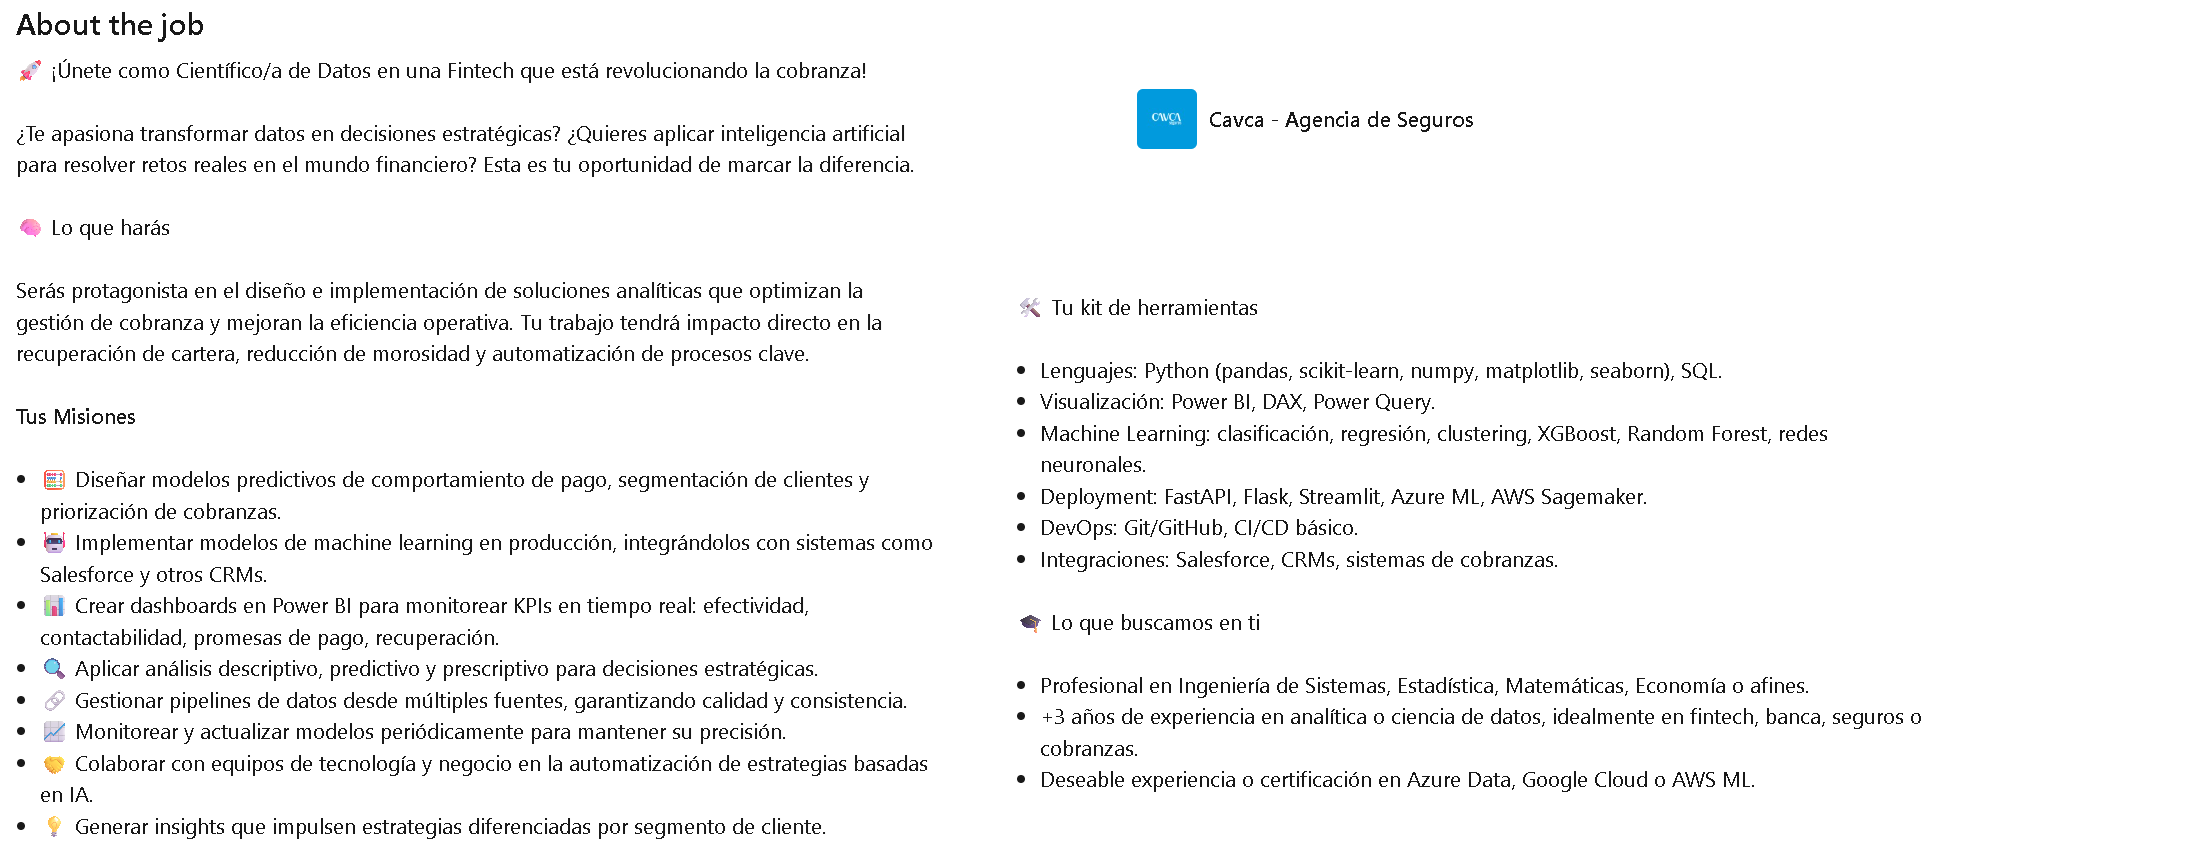
\includegraphics[width=1\linewidth,height=\textheight,keepaspectratio]{assets/TrabajoDataScientist.png}
Tomado de Linkedin

\subsection{Roles Orientados a Datos}\label{roles-orientados-a-datos}

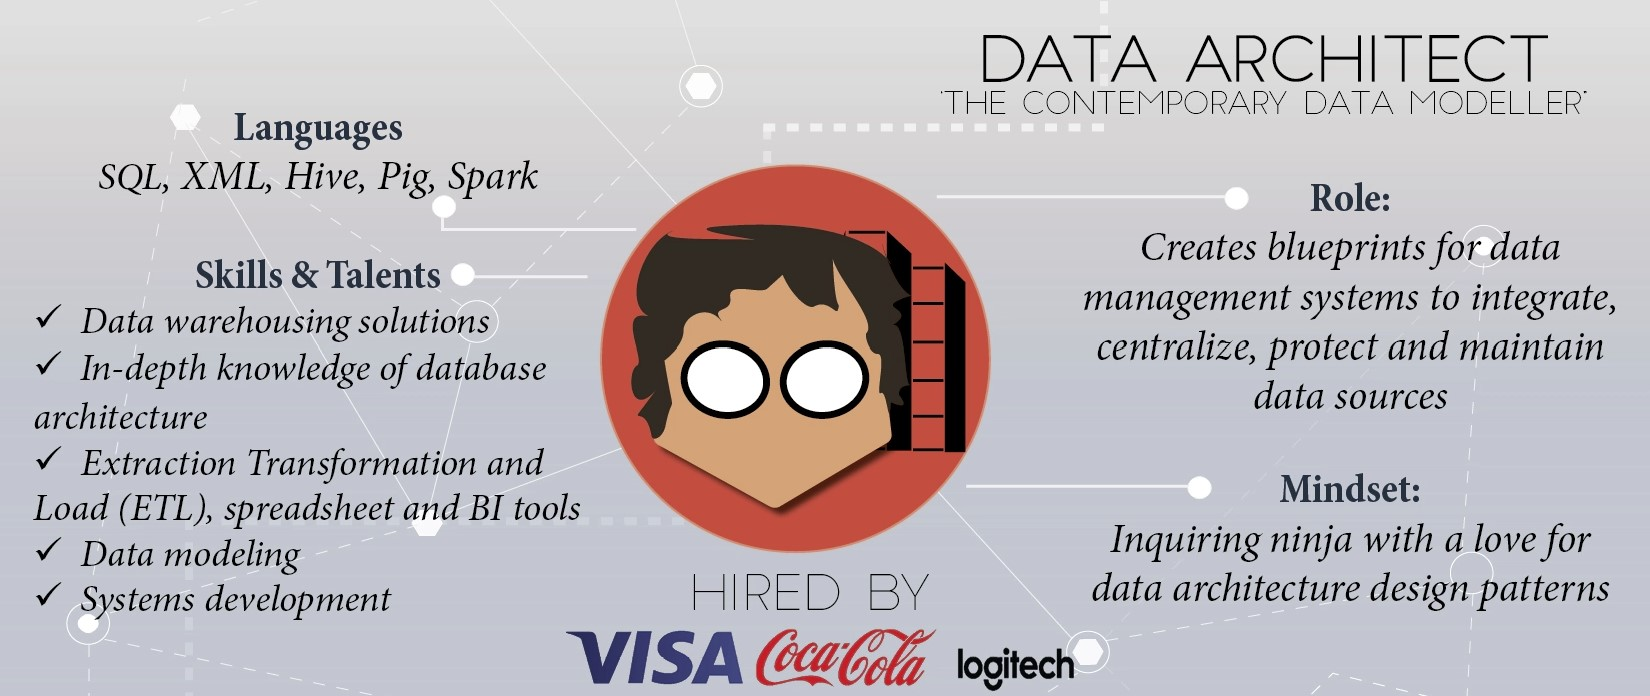
\includegraphics[width=1\linewidth,height=\textheight,keepaspectratio]{assets/dataArchitect.jpg}
Tomado de:
\url{https://www.datacamp.com/tutorial/data-science-industry-infographic}

\subsection{Roles Orientados a Datos}\label{roles-orientados-a-datos-1}

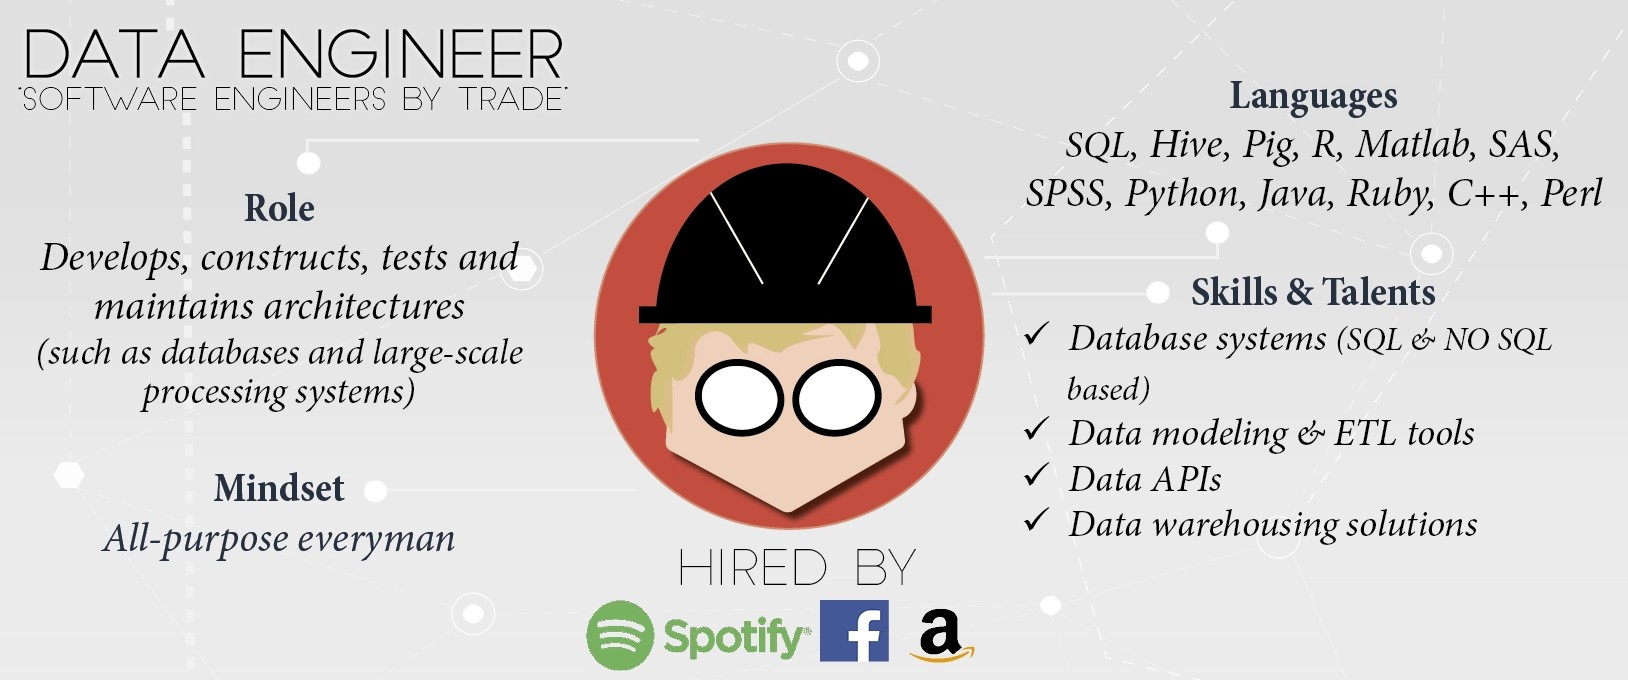
\includegraphics[width=1\linewidth,height=\textheight,keepaspectratio]{assets/dataEngineer.jpg}
Tomado de:
\url{https://www.datacamp.com/tutorial/data-science-industry-infographic}

\subsection{Remuneración}\label{remuneraciuxf3n}

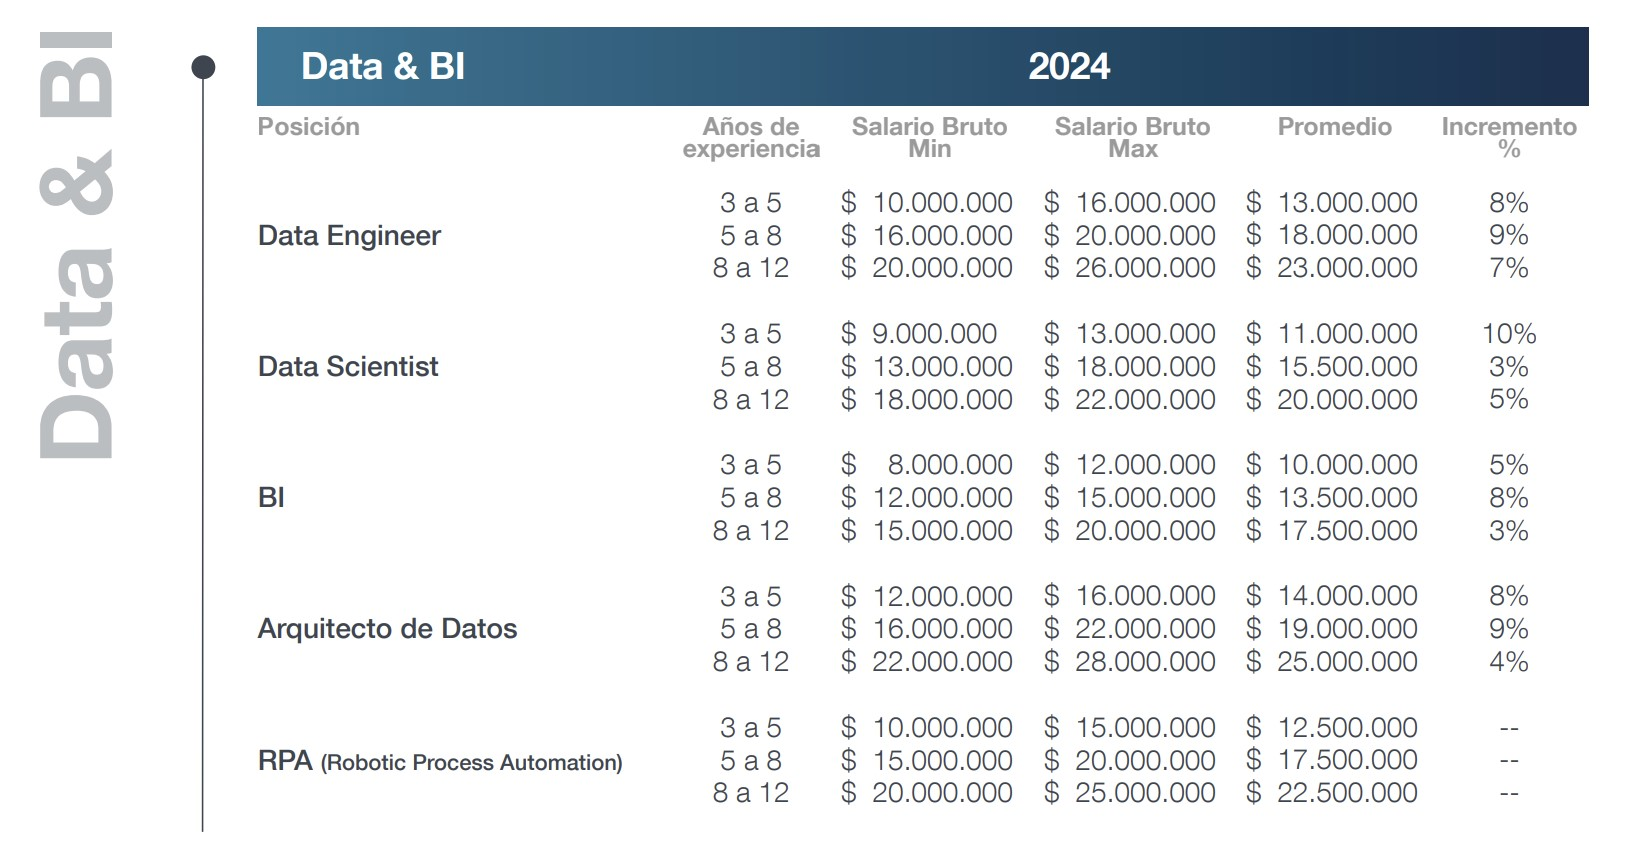
\includegraphics[width=0.8\linewidth,height=\textheight,keepaspectratio]{assets/EstudioRemuneracion.jpg}
Tomado de:
\url{https://www.michaelpage.com.co/estudios-y-tendencias/estudio-de-remuneracion-tecnologia-2024-1-IT-088}

\subsection{Remuneración}\label{remuneraciuxf3n-1}

\textbf{Pregunta}

¿Saben por qué el mercado paga entre 13 y 20 millones de pesos a un
junior en estos roles?

\begin{verbatim}
 Tomado de: [https://www.michaelpage.com.co/estudios-y-tendencias/estudio-de-remuneracion-tecnologia-2024-1-IT-088](https://www.michaelpage.com.co/estudios-y-tendencias/estudio-de-remuneracion-tecnologia-2024-1-IT-088)
\end{verbatim}

\subsection{Objetivos de Formación}\label{objetivos-de-formaciuxf3n}

\begin{itemize}
\tightlist
\item
  \textbf{Herramientas Prácticas:} Brindar herramientas de Machine
  Learning para el desarrollo de soluciones a problemas reales.
\item
  \textbf{Desarrollo de Habilidades:} Aplicar conceptos fundamentales
  para fortalecer la capacidad de abstracción y la resolución de
  problemas.
\item
  \textbf{Conciencia Crítica:} Generar reflexión sobre el impacto social
  y las implicaciones éticas del Machine Learning.
\end{itemize}

\subsection{Resultados de Aprendizaje
Esperados}\label{resultados-de-aprendizaje-esperados}

Al finalizar el curso, el estudiante podrá: - \textbf{Resolver
Problemas:} Aplicar principios de Machine Learning para solucionar
problemas en su campo profesional. - \textbf{Validar Soluciones:}
Diseñar experimentos para evaluar la efectividad de las soluciones
implementadas. - \textbf{Actuar con Ética:} Discutir y aplicar la
responsabilidad ética y social en el uso de la tecnología, fomentando el
autoaprendizaje.

\subsection{Libros - Ética en IA}\label{libros---uxe9tica-en-ia}

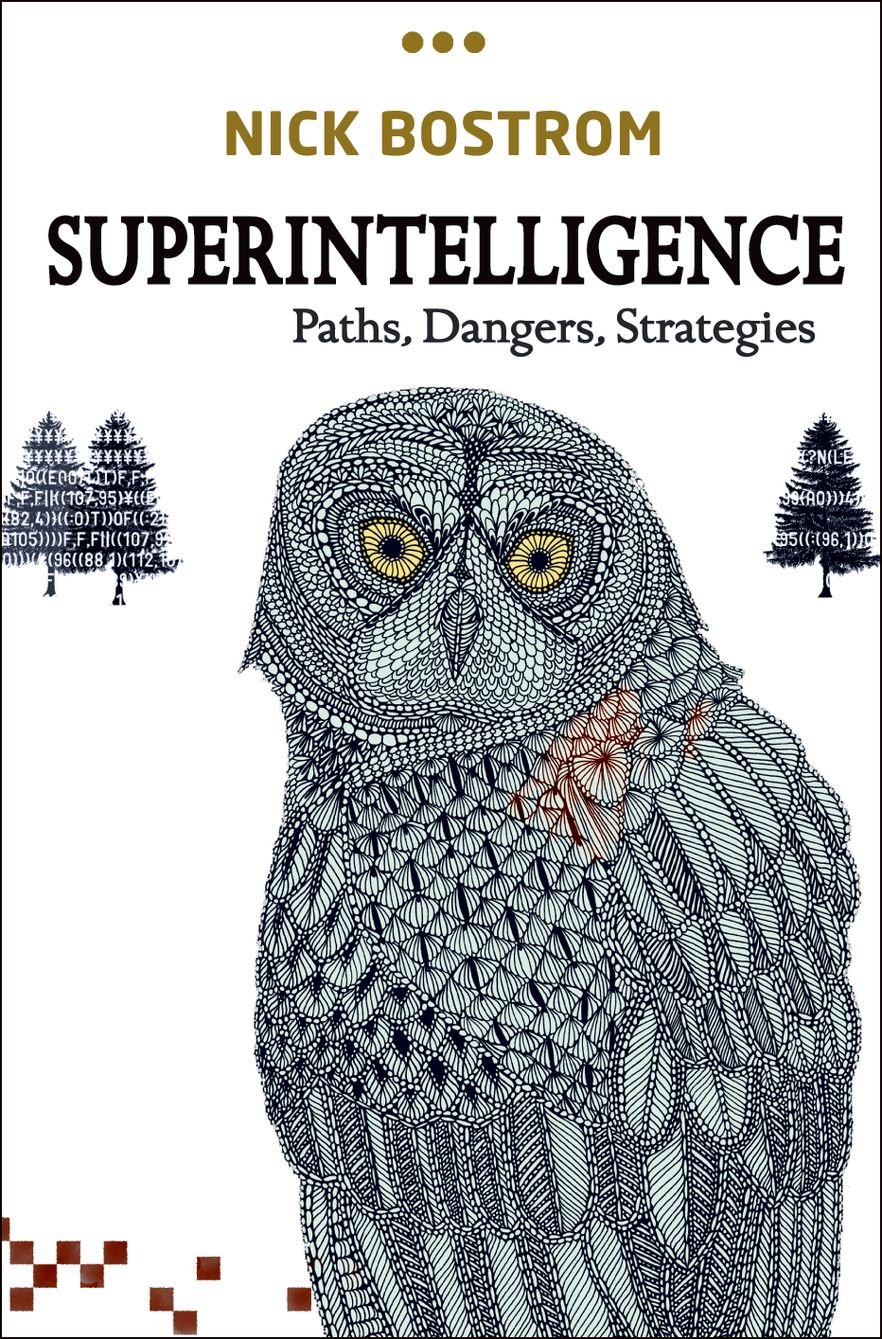
\includegraphics[width=0.3\linewidth,height=\textheight,keepaspectratio]{assets/SuperIntelligence.jpg}\\

\includegraphics[width=0.3\linewidth,height=\textheight,keepaspectratio]{assets/WeaponsMath.jpg}


\includegraphics[width=0.3\linewidth,height=\textheight,keepaspectratio]{assets/Nexus.jpg}

\section{Aprendizaje de Máquina}\label{aprendizaje-de-muxe1quina-1}

\section{Herramientas}\label{herramientas}

\subsection{Popularidad de los lenguajes de
programación}\label{popularidad-de-los-lenguajes-de-programaciuxf3n}

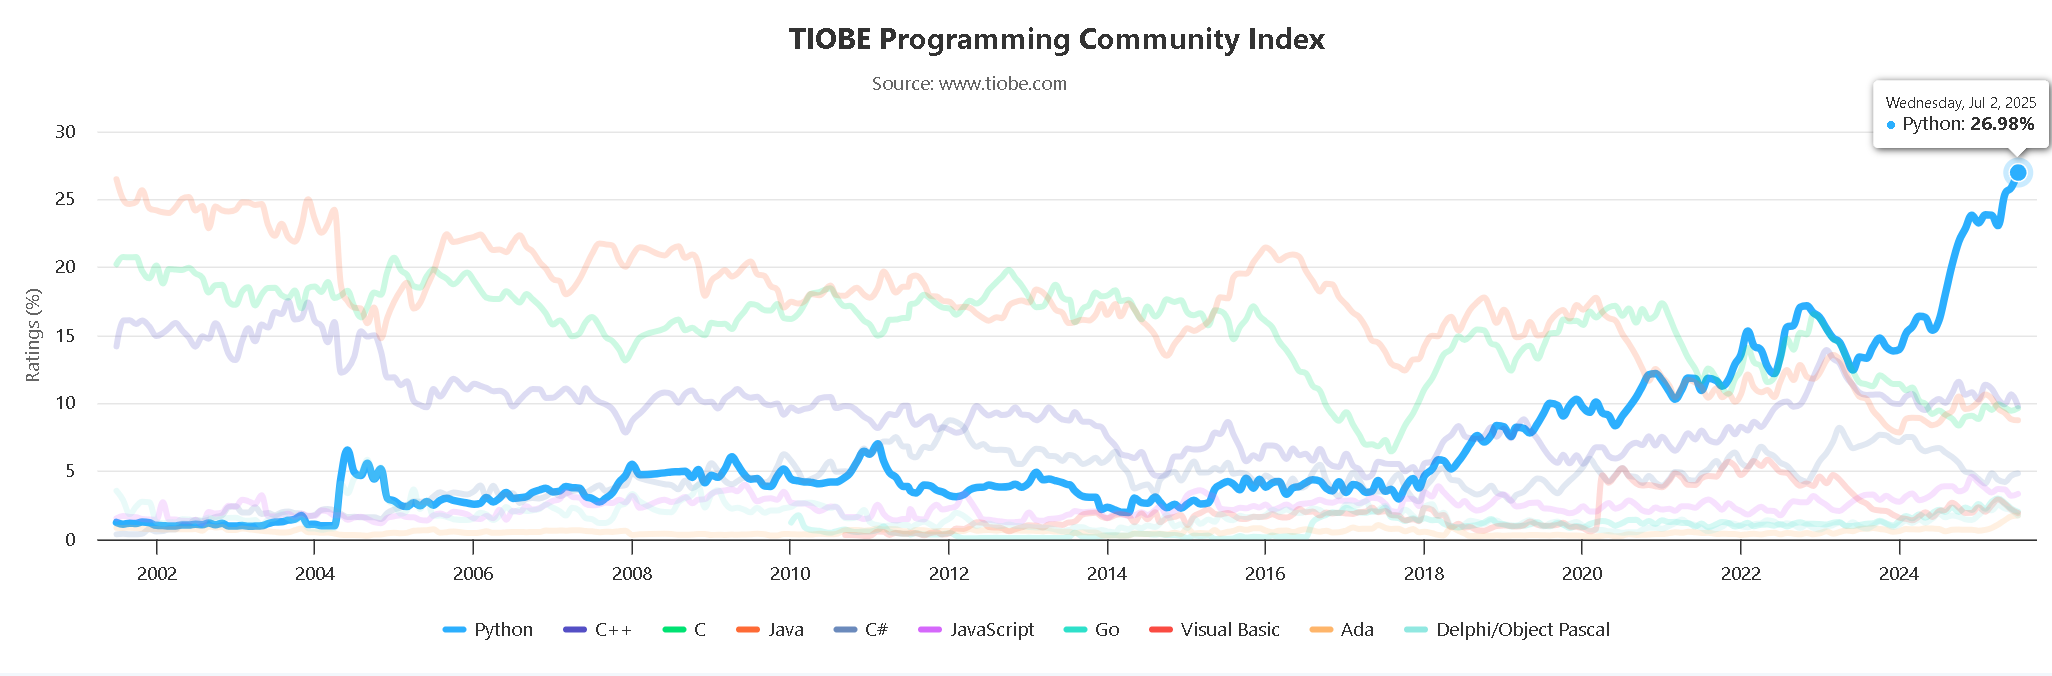
\includegraphics[width=1\linewidth,height=\textheight,keepaspectratio]{assets/Python.png}
Tomado de \url{https://www.tiobe.com/tiobe-index/}

\subsection{Sklearn y Problemas de ML}\label{sklearn-y-problemas-de-ml}

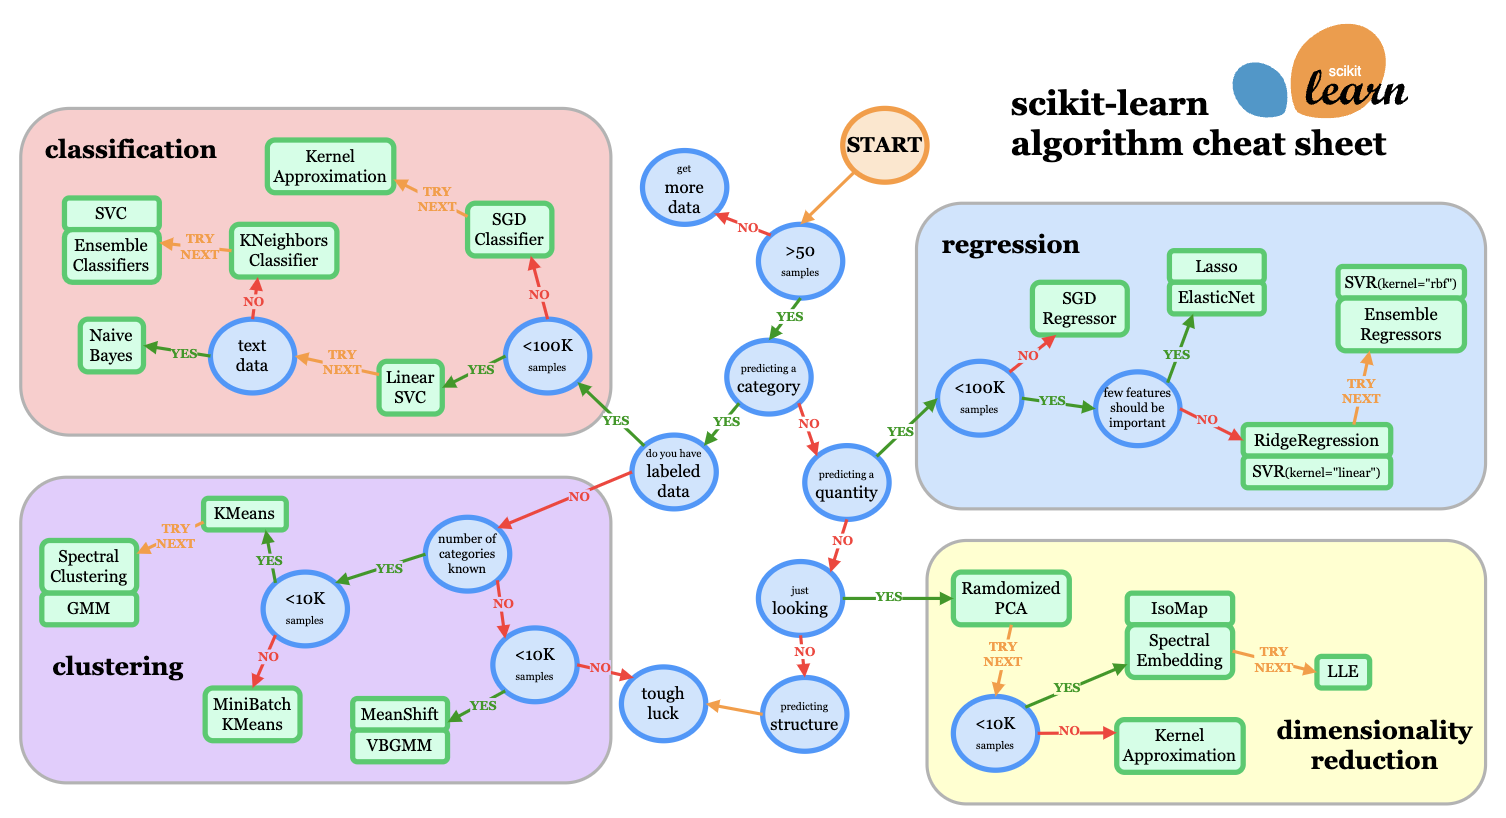
\includegraphics[width=0.9\linewidth,height=\textheight,keepaspectratio]{assets/selectingAlgo.png}

\subsection{Herramientas Sugeridas}\label{herramientas-sugeridas}

\begin{table}[h]


| **Nombre** | **Descripción** | **Enlace** |
| --- | --- | --- |
| Google Colab | Herramienta de ambiente de ejecución en la nube para documentar y ejecutar código Python | [https://colab.research.google.com](https://colab.research.google.com) |
| Google Gemini | Modelo LLM para aprendizaje de programación Python | [https://gemini.google.com/](https://gemini.google.com/) |
| N8N | Plataforma de desarrollo de workflows | [https://n8n.io/](https://n8n.io/) |

\caption{Herramientas de IA}
\end{table}

\subsection{Google Colab}\label{google-colab}

Ambiente de desarrollo en Python o R para el análisis de datos. Permite
la ejecución en la nube de programas, con una cantidad generosa de
recursos.

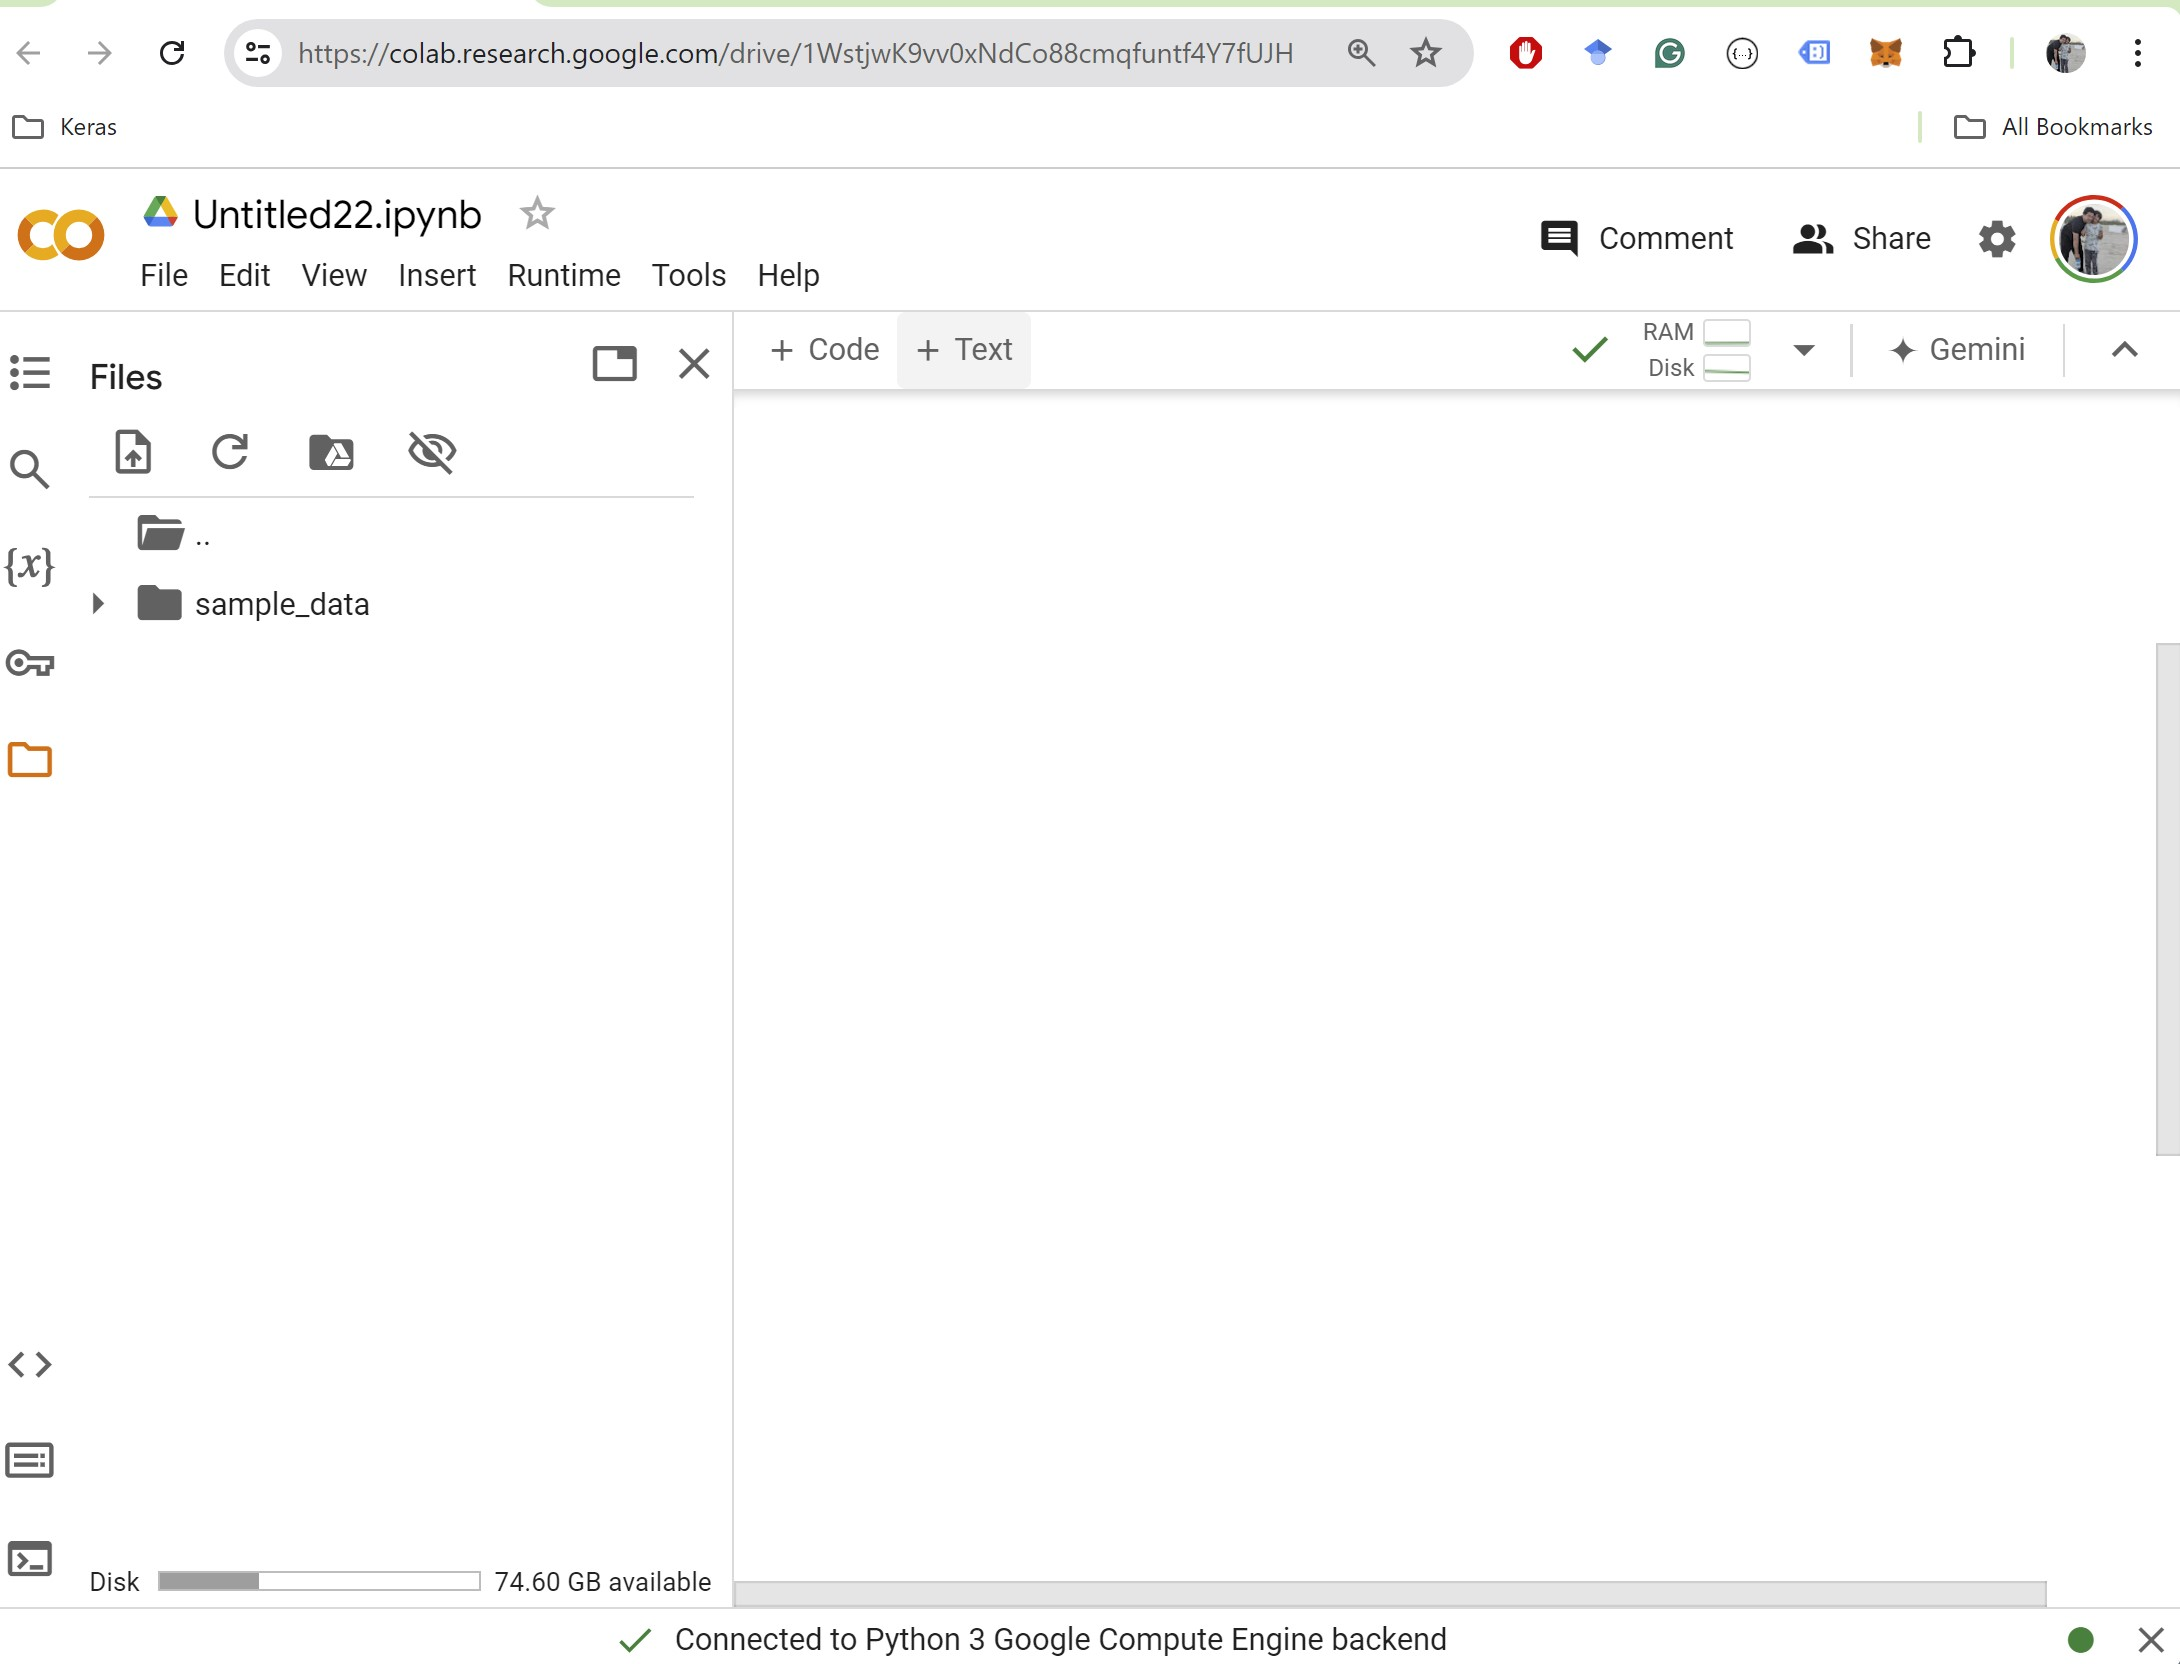
\includegraphics[width=1\linewidth,height=\textheight,keepaspectratio]{assets/colabIDE.jpg}

\subsection{Google Colab con Gemini}\label{google-colab-con-gemini}

Cuenta con el chat de Gemini embebido en el ambiente de desarrollo.
Asiste en la escritura de código.

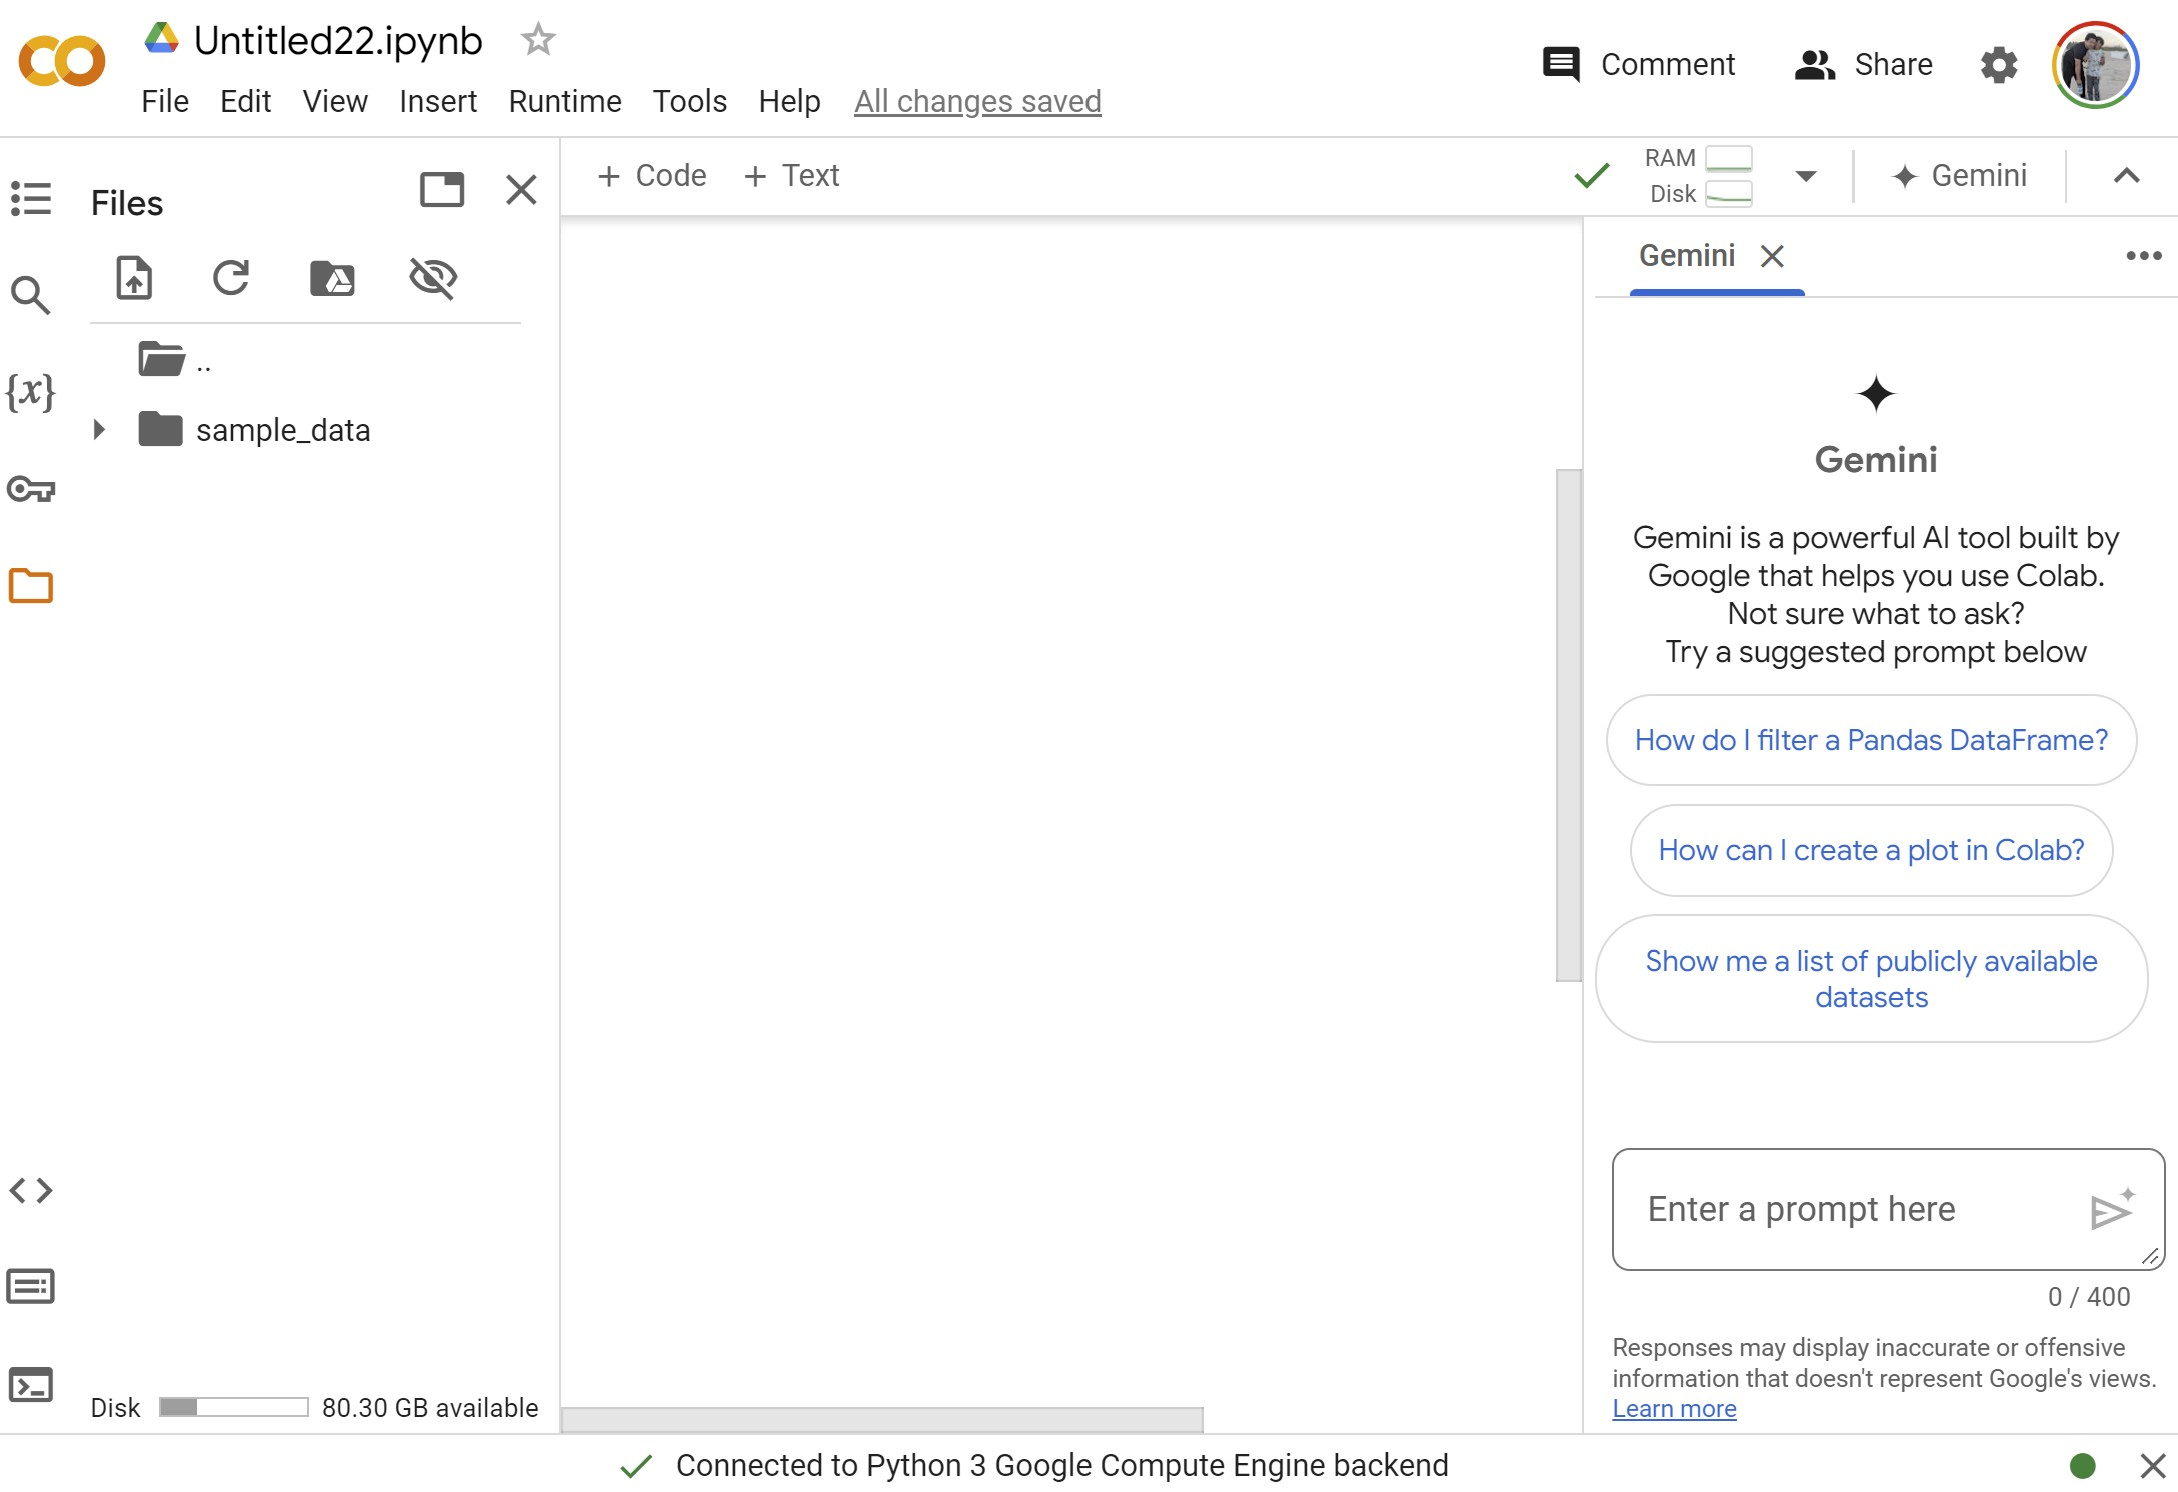
\includegraphics[width=1\linewidth,height=\textheight,keepaspectratio]{assets/colabIDEGemini.jpg}

\subsection{Análisis Exploratorio de
Datos}\label{anuxe1lisis-exploratorio-de-datos}

\textbf{Prompt}: Haz un analisis exploratorio de datos del archivo de
github datasciencedojo titanic.csv usando la librería ydata-profiling.
Instala la ultima version disponible de la libreria.

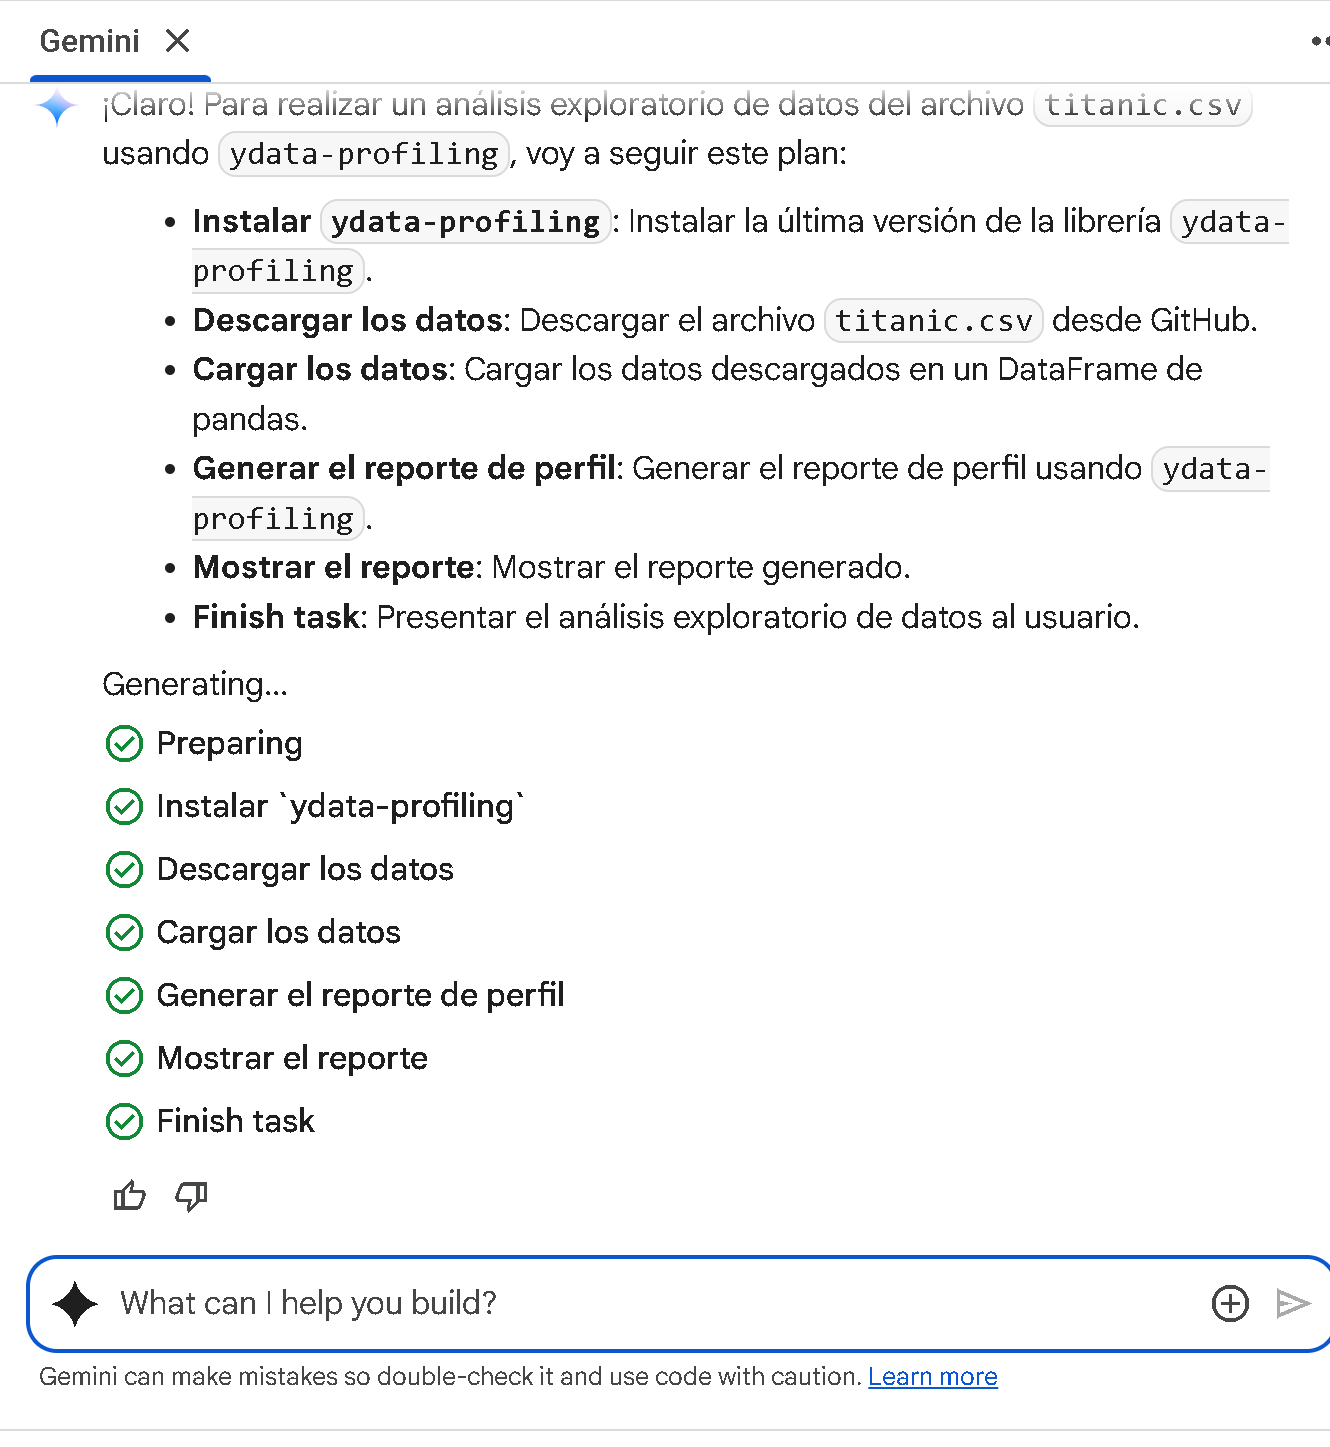
\includegraphics[width=1\linewidth,height=\textheight,keepaspectratio]{assets/ColabAgentico.png}

\subsection{Análisis Exploratorio de
Datos}\label{anuxe1lisis-exploratorio-de-datos-1}

\textbf{Prompt}: Haz un analisis exploratorio de datos del archivo de
github datasciencedojo titanic.csv usando la librería ydata-profiling.
Instala la ultima version disponible de la libreria.

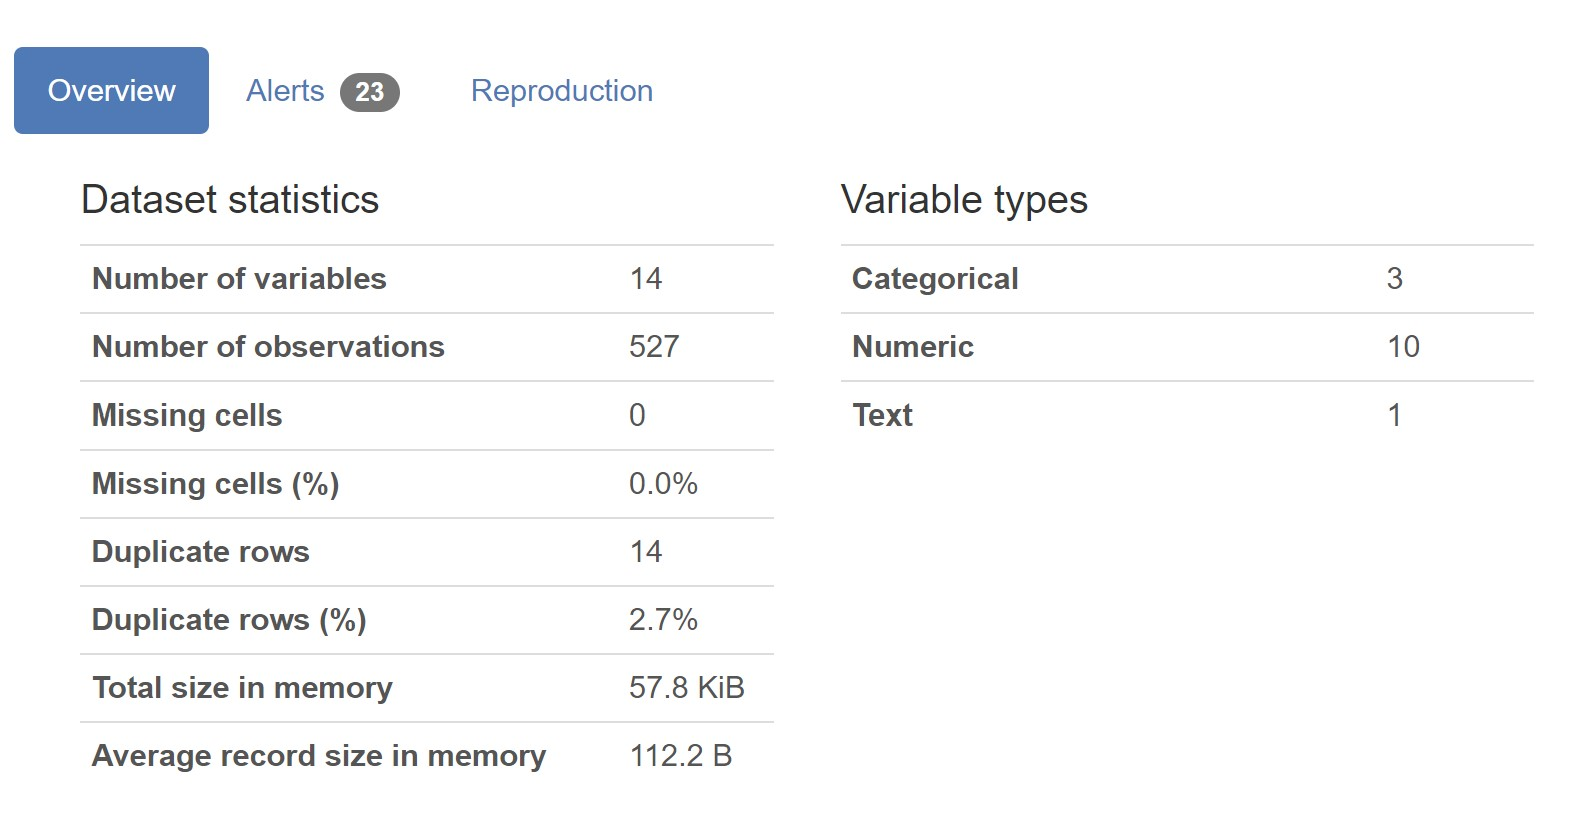
\includegraphics[width=1\linewidth,height=\textheight,keepaspectratio]{assets/colabYdata.jpg}

\nocite{*}

\subsection{References}\label{references}

\AtNextBibliography{}
\printbibliography

\protect\phantomsection\label{refs}
\begin{CSLReferences}{1}{1}
\bibitem[\citeproctext]{ref-geron2022hands}
Géron, Aurélien. 2022. \emph{Hands-on Machine Learning with
Scikit-Learn, Keras, and TensorFlow: Concepts, Tools, and Techniques to
Build Intelligent Systems}. 3rd ed. O'Reilly Media, Inc.

\bibitem[\citeproctext]{ref-russell_norvig_2020}
Russell, Stuart J., and Peter Norvig. 2020. \emph{Artificial
Intelligence: A Modern Approach}. 4th ed. Pearson.

\end{CSLReferences}




\end{document}
